\documentclass[12pt]{article}
\usepackage{packages}
\begin{document}
\begin{center}
  
{\Large {\bf Algoritmos de Aproximação para \\Problemas de Clustering}
}

\vspace{0.2cm}
{\small 
{\bf Orientadora:} Cristina Gomes Fernandes \\
{\bf Aluno:} João Guilherme Alves Santos
}

\vspace{5mm} 

\begin{abstract}
Este é o texto escrito durante a iniciação científica do aluno de graduação João Guilherme Alves Santos, financiado pelo projeto FAPESP 2023/16197-0, sob supervisão da Profa.\ Dra.\ Cristina Gomes Fernandes.
\end{abstract}

\end{center}
\newpage

\tableofcontents
\newpage

\section{Introdução}

Problemas de otimização têm o objetivo de encontrar um ponto ótimo de uma função definida sobre um certo domínio. Especificamente, os problemas de otimização combinatória têm domínio finito. Muitos desses problemas são $\NP$-difíceis. Para problemas $\NP$-difíceis, não existem algoritmos eficientes que encontrem uma solução ótima para toda instância de tais problemas a menos que $P = \NP$.

Nesse contexto, algoritmos de aproximação surgiram. A ideia é abrir mão de encontrar soluções ótimas para encontrar, eficientemente, uma solução cujo valor garante uma relação pré-estabelecida com o valor ótimo. 

Clustering refere-se a uma classe de problemas de otimização cujo objetivo é agrupar objetos de maneira que objetos no mesmo cluster apresentem mais semelhanças quando comparados a objetos em clusters diferentes. Tais semelhanças serão definidas pelo problema em questão. Neste projeto, iremos estudar, sob o ponto de vista de algoritmos de aproximação, três problemas de clustering $\NP$-difíceis: localização de instalações, $k$-mediana e $k$-centros. 

Localização de instalações é um problema que visa determinar a melhor localização para instalações, como fábricas ou depósitos, com base no custo de abertura das instalações e custos de transporte. Além disso, pode ser modelado para outras aplicações como problemas de posicionamento de caches em um computador ou problemas de projeto de redes.
Existem várias versões do problema de localização de instalações, a mais simples delas é a versão sem capacidades em que as instalações não têm limitações para suprir os clientes.

No problema de localização de instalações sem capacidades, temos um grafo $(F,D)$-bipartido completo em que $D$ é o conjunto de clientes a serem atendidos e $F$ o conjunto de instalações que podem ser abertas. Para cada cliente $j \in D$ e cada instalação $i \in F$, há um custo $c_{ij}$ para a aresta $ij$ em associar o cliente $j$ à instalação $i$. Além disso, existe um custo de abertura $f_i$ para cada instalação $i \in F$. Seja $F' \subseteq F$, uma associação referente a $F'$ é uma função $\sigma : D \to F'$. Definimos o custo para $F'$ e $\sigma$ como $\text{custo}(F',\sigma)\coloneqq \sum_{ i \in F'} f_i + \sum_{j \in D} c_{\sigma_{j}j}$. Além disso, definimos custo$(F') \coloneqq~\min_{\sigma}~\text{custo}(F',\sigma)$. Claramente, o $\sigma^*$ que minimiza isso é $\sigma^*(j) = \min_{i \in F'} c_{ij}$, para todo $j \in D$. Assim, o objetivo do nosso problema é encontrar um subconjunto $F' \subseteq F$ que minimize custo$(F')$.

%O objetivo do problema é escolher um conjunto $F' \subseteq F$ tal que o custo total de abertura das instalações em $F'$ somado ao custo de associação de cada cliente $j \in D$ à instalação em $F'$ mais próxima a ele seja minimizado. Para uma solução qualquer $S$, definimos a função $\sigma_S : D \to F$ como $\sigma_S(j) = \arg\min_{i \in S}$ c_{ij} para todo $j \in D$. Assim, o custo da solução $S$ é custo$(S) = \sum_{i \in S} f_i + \sum_{j \in $. Em outras palavras, queremos encontrar $F' \subseteq F$ e uma função $\sigma$ que minimize $\sum_{i\in F'} f_i + \sum_{j \in D} c_{\sigma(j)j}$. 

O problema $k$-mediana é muito parecido com o problema de localização de instalações. A diferença aqui é que não temos custo para a abertura de instalações, mas podemos abrir no máximo $k$ delas. 
Assim como no localização de instalações, no problema $k$-mediana temos um grafo $(F,D)$-bipartido completo em que $D$ é o conjunto de clientes a serem atendidos e $F$ o conjunto de instalações que podem ser abertas. Para cada cliente $j \in D$ e cada instalação $i \in F$, há um custo $c_{ij}$ para a aresta $ij$ em associar o cliente $j$ à instalação $i$. Temos também um inteiro $k$ que representa a quantidade de instalações que podem ser abertas. Então, queremos encontrar um conjunto $F' \subseteq F$ de tamanho $k$ e uma função que associe cada cliente a uma instalação aberta tal que o custo total de associação seja minimizado.

No problema dos $k$-centros não existe essa diferença entre instalações que podem ser abertas e clientes, teremos cidades e escolheremos $k$ delas para construir instalações.
Então, temos um grafo $G(V,E)$ completo em que $V$ são cidades e temos um custo $c_{e}$ para associar as cidades que são extremos de $e$. Temos também um inteiro $k$ que representa a quantidade de cidades em que uma instalação será aberta. Cada cidade será associada a uma cidade com uma instalação aberta com menor custo de associação entre elas. O objetivo do nosso problema é minimizar o maior custo de associação entre uma cidade qualquer e a cidade a qual ela está associada.

Diversos métodos podem ser utilizados para aproximar o problema de localização de instalações. Charikar e Guha desenvolveram um algoritmo com razão de aproximação $2.414$ utilizando o método de busca local~\cite{Charikar&Guha'05}.  Esse problema também pode ser modelado como um problema de programação inteira e, por isso, técnicas envolvendo programação linear podem ser aplicadas a ele.  Por exemplo, há algoritmos que fazem o arredondamento de soluções da relaxação linear do programa inteiro para obter uma solução aproximada do problema.  Alguns destes algoritmos atingem boas razões de aproximação, por exemplo, chegando a 1.677~\cite{Byrka&Aardal'10}. Entretanto, a melhor aproximação encontrada utiliza de vários métodos, incluindo o conhecido método primal-dual, e garante uma razão de aproximação 1.488~\cite{LI'13}. Essa não é muito distante do melhor que se poderia encontrar, uma vez que Guha e Khuller mostraram que não existe algoritmo para esse problema com razão de aproximação melhor que 1.463~\cite{GUHA1999228}, a menos que $P = \NP$.


Dentre os três problemas apresentados, o $k$-mediana é o que tem a maior folga entre o melhor resultado de inaproximabilidade e a razão do melhor algoritmo de aproximação conhecido. Jain, Mahdian e Saberi provaram que não existe algoritmo polinomial com razão de aproximação $1+ \frac{2}{e}$ para o $k$-mediana~\cite{JMS'02}, assumindo que $P \neq \NP$, enquanto a melhor aproximação encontrada tem razão $2.675 + \epsilon$~\cite{BPRST'17}.


Hsu e Nemhauser~\cite{HSU1979209} mostraram que não existe algoritmo polinomial com razão de aproximação menor que 2 para o problema dos $k$-centros, assumindo que $P\neq\NP$. Neste caso, temos algoritmos que apresentam o melhor desempenho possível: utilizando o método do gargalo, Gonzalez~\cite{GONZALEZ1985293} e independentemente Hochbaum e Shmoys~\cite{HochShmoys'85} desenvolveram um algoritmo polinomial com razão de aproximação igual a 2.

% \newpage
\section{$k$-Centros}
    Seja $I(G,c,k)$ uma instância do problema dos $k$-centros e $C \subseteq V$ uma solução viável para $I$. Vamos definir alguns termos que facilitarão as explicações seguintes. Os vértices de $C$ serão chamados \emph{centros de cluster}. Os vértices de $V$ serão particionados em $k$ conjuntos chamados \emph{clusters} e cada um deles terá exatamente um centro de cluster. Um vértice estará no mesmo cluster que um centro de cluster associado a ele. Cada cluster terá um \emph{raio} que é o maior custo entre o seu centro e um vértice qualquer dele. O nosso problema se resume a encontrar um conjunto $C$ que minimize o maior desses raios. Denotamos por raio$(C)$ o maior raio de um cluster induzido por $C$.

Antes de falarmos sobre algoritmos de aproximação para o problema dos $k$-centros, vamos mostrar que, assumindo $P\neq\NP$, não existe algoritmo polinomial que resolva nosso problema, ou seja, vamos mostrar que nosso problema é $\NP$-difícil. Para isso, vamos definir o problema do $k$-conjunto dominante.

\begin{definition}
    Seja $G = (V,E)$ um grafo. Um conjunto $D \subseteq V$ é chamado \emph{dominante} se, para todo vértice $u \in V \setminus D$, existe um vértice $v \in D$ tal que $uv \in E$.
\end{definition}

\begin{problem}[$k$-conjunto dominante]
    Dado um grafo $G$ e um inteiro $k$, decidir se $G$ tem um conjunto dominante $D$ tal que $|D| \leq k$.      
\end{problem}
Esse problema é $\NP$-completo, sendo o problema GT2 do famoso livro de Garey e Johnson~\cite{garey1979computers}. Usaremos este problema para mostrar que o problema dos $k$-centros é $\NP$-difícil.

\begin{theorem}\label{theorem:2.3}
    O problema dos $k$-centros para instâncias métricas é $\NP$-difícil.
\end{theorem}

\begin{proof}
    Suponha que exista um algoritmo $A$ que resolve o problema dos $k$-centros em tempo polinomial. Seja $G = (V,E)$ um grafo e $I(G,k)$ uma instância do problema $k$-conjunto dominante. Vamos criar uma instância $I'(G',c,k)$ do problema dos $k$-centros a partir da instância $I$. A instância $I'$ tem como grafo $G'(V,E')$ completo tal que, para todo $e \in E'$,
    \[
    c_e = \begin{cases}
            1, \text{ se } e \in E \\
            2, \text{ caso contrário.} 
            \end{cases}\]\\
    Note que $c$ satisfaz a desigualdade triangular e pode ser obtida de $I$ em tempo polinomial.

    O algoritmo aplicado à instância $I'$ encontra uma solução $C$, ou seja, um conjunto de $k$ centros de cluster. Se raio$(C)=1$ então todos os vértices estão ligados ao centro do seu cluster com uma aresta de $G$ e assim $C$ é um conjunto dominante em $G$. 
    Como o algoritmo $A$ minimiza o raio de $C$, se raio$(C)=2$, não existe uma solução para $I'$ em que os vértices estejam ligados ao centro do seus clusters apenas por arestas de $G$ e, por isso, não existe um conjunto dominante de tamanho menor ou igual a $k$ em $G$.

    Portanto, conseguimos resolver em tempo polinomial o problema do $k$-conjunto dominante, o que implicaria que $P = \NP$.
\end{proof}

O resultado acima pode ser adaptado para dar um resultado mais forte de inaproximabilidade para a versão geral do problema, não restrita à métrica.
\begin{theorem}
    Seja $\alpha(n)$ uma função computável com $\alpha(n)\geq 1$ para todo $n$. Não existe $\alpha(n)$-aproximação para a versão geral do $k$-centros, onde $n$ é o número de vértices do grafo da instância, a menos que $P=\NP$.
\end{theorem}

\begin{proof}
        A demonstração desse teorema é muito parecida com a do Teorema~\ref{theorem:2.3}. \\
        Seja $G = (V,E)$. Suponha que exista um algoritmo polinomial $A$ que é uma $\alpha(n)$-aproximação do $k$-centros e seja $I(G,k)$ uma instância do problema do $k$-conjunto dominante em que $G$ tem $n$ vértices. Vamos criar uma instância $I'(G',c,k)$ do problema dos $k$-centros a partir da instância $I$. A instância $I'$ tem como grafo $G'(V,E')$ completo tal que, para cada $e \in E'$, \\
    \[c_e = \begin{cases}
            1, \text{ se } e \in E \\
            \alpha(n)+1, \text{ caso contrário.} 
            \end{cases}\]\\
    Como $\alpha(n)$ é uma função computável, essa instância pode ser construída a partir de $I$ em tempo polinomial.
    Se $\alpha(n)=1$, então $c$ obedece a desigualdade triangular e $A$ é um algoritmo polinomial e exato, o que, pelo Teorema~\ref{theorem:2.3}, é absurdo. Então, suponha $\alpha(n)>1$.

    O algoritmo aplicado à instância $I'$ encontra uma solução $C$ de tamanho $k$. Como $c_e = 1$ ou $\alpha(n)+1$ para todo $e \in E'$, então raio$(C)=1$ ou $\alpha(n)+1$.
    Se raio$(C)=1$ então todos os vértices estão ligados ao centro do seu cluster com aresta de $G$, e assim $C$ é um conjunto dominante em $G$.
    Se raio$(C) = \alpha(n) + 1$, então $\opt(I) \geq \frac{\alpha(n)+1}{\alpha(n)}>1$. Assim, não existe solução $C'$ tal que raio$(C')=1$ e não existe $k$-conjunto dominante em $G'$ que utilize apenas arestas de $G$.

    Portanto, conseguimos resolver o problema do $k$-conjunto dominante em tempo polinomial o que, assumindo que $P \neq \NP$, é um absurdo.
\end{proof}
    Fica, então, explícita a impossibilidade de encontrarmos algoritmos de aproximação para a versão geral do problema dos $k$-centros, a menos que $P = \NP$\\
    Agora que justificamos o estudo de algoritmos de aproximação para esse problema vamos mostrar um limitante inferior para a razão de aproximação desses algoritmos.
    
    \begin{theorem}
        Seja $\varepsilon \in (0,1]$. Não existe $(2-\varepsilon)$-aproximação para o problema dos $k$-centros, a menos que $P=\NP$.
    \end{theorem}
    A prova do Teorema~\ref{theorem:2.3} essencialmente serve também para esse Teorema, a única diferença é que aqui precisamos assumir a existência de um algoritmo que é uma $(2 - \varepsilon)$-aproximação para o problema dos $k$-centros.

    Começaremos por um algoritmo simples, mas que garante a melhor razão de aproximação.
% \newpage

\subsection{Algoritmo guloso}
    Nessa seção vamos falar sobre o algoritmo guloso para o problema dos $k$-centros. Esse algoritmo foi desenvolvido pelo González~\cite{GONZALEZ1985293} e foi estudado na Seção 2.2 do livro WS2011.

Seja $G \coloneqq (V,E)$ o grafo da instância do problema e $c_e$ o custo de uma aresta $e \in E$.
Definimos a função $c(u,S)$ que é definida para um vértice $u$ e um conjunto $S$ de vértices  por,
\[ c(u,S) \coloneqq \min_{v\in S} c_{uv}
    \]
A ideia desse algoritmo guloso se concentrará em, a cada iteração, escolher o vértice $u$ tal que $c(u,C)$ seja o maior possível, sendo $C$ o conjunto dos centros de cluster escolhidos até aquele momento.

\begin{algorithm}
\caption{\sc Guloso-González$(G,c,k)$}
    \label{k-center:guloso}
    \begin{algorithmic}[1]
  \State Escolha arbitrariamente $u \in V$.
        \State $C \gets \{u\}$.
        \While{$|C| \leq k$}
        \State $v \gets \arg\max_{j \in V} c(j,C)$
        \State $C \gets C \cup \{v\}$
        \EndWhile
  \State Devolva $C$.
\end{algorithmic}
\end{algorithm}

\begin{theorem}
    O algoritmo {\sc Guloso-González}$(G,c,k)$ é uma $2$-aproximação do problema dos $k$-centros.
\end{theorem}
\begin{proof}
    É evidente que o algoritmo roda em tempo polinomial. 
  
    Seja $C^*$ uma resposta ótima de $I(G,c,k)$ e $C$ uma resposta devolvida pelo algoritmo {\sc Guloso-González}. Vamos mostrar que raio$(C) \leq 2\text{raio}(C^*) $. Perceba que o custo de uma aresta entre dois vértices quaisquer de um mesmo cluster de $C^*$ é no máximo $2\opt(I)$, uma vez que vale a desigualdade triangular.
    Se há um vértice de $C$ em cada cluster de $C^*$, todos os vértices estão ligados com uma aresta de custo no máximo $2\opt(I)$ a um centro de cluster de $C$. Então raio$(C) \leq 2\opt(I)$. Senão, suponha sem perda de generalidade que $C_{i-1} \coloneqq \{ u_1,u_2,\ldots,u_{i-1}\}$ é o $C$ ao final da iteração $i-1$ e cada $u_j$ está em um cluster diferente de $C^*$. Seja $u_i$ o vértice escolhido na iteração $i$ e suponha que ele está no mesmo cluster que um vértice $u_j$ para algum $j=1,\ldots,i-1$. Então, $c(u_i,C_{i-1}) \leq c(u_iu_j) \leq 2\opt(I)$. Como $u_i$ maximiza $c(v,C_{i-1})$, então raio$(C) \leq 2\opt(I)$.
\end{proof}

Vamos mostrar que essa análise é justa, ou seja, existe uma instância $I(G,c,k)$ em que o algoritmo devolve uma solução $C$ tal que raio$(C) = 2 \opt(I)$. 

Seja $G$ um grafo com pelo menos $k+2$ vértices em que as arestas têm custo 1 ou~2. O grafo induzido pelas arestas de custo 1 é uma estrela, como mostrado na figura abaixo.
\[
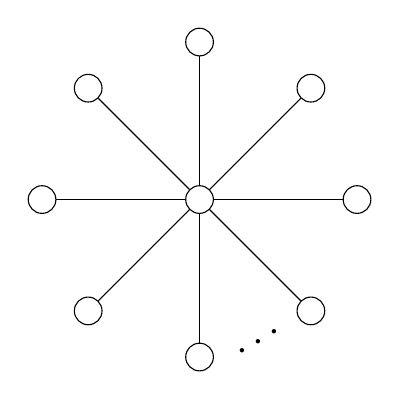
\begin{tikzpicture}
    % Number of outer vertices in the star
    \def\n{8}
    
    % Radius of the star
    \def\r{2cm}
    
    % Rotation angle
    \def\rotationangle{90}
    
    % Draw the central vertex
    \draw (0,0) node[circle, draw, minimum size=10pt, inner sep=1.5pt] (center) {};
    
    % Draw the outer vertices, rotated
    \begin{scope}[rotate=\rotationangle]
      \foreach \i in {1,...,\n} {
        \draw (\i*360/\n:\r) node[circle, draw, minimum size=10pt, inner sep=1.5pt] (\i) {};
      }
    \end{scope}
    
    % Connect the central vertex to every outer vertex
    \foreach \i in {1,...,\n} {
      \draw (center) -- (\i);
    }
    \draw (4) node[shift={(0.75,0.2)}] {\rotatebox{30}{\scalebox{1.5}{$\ldots$}}} (4);
  \end{tikzpicture}
  \]

  Claramente, o raio de uma resposta ótima dessa instância é 1 e inclui o vértice do centro da estrela como um dos centros de cluster.
  Note que se, no algoritmo guloso, o vértice escolhido arbitrariamente for algum dos vértices da ponta dessa estrela o vértice do centro nunca será escolhido, uma vez que ele nunca maximizará a função $c(j,C)$. Assim, serão escolhidos apenas vértices da ponta da estrela e como temos pelo menos $k+1$ delas, sempre existirá um vértice ligado ao centro do seu cluster com uma aresta de custo 2.
% \newpage

\subsection{Método do gargalo}
    Os chamados problemas de gargalo são aqueles definidos em grafos com pesos nas arestas tais que a resposta ótima é o peso de uma aresta.

Para o próximo algoritmo será necessário saber o que é um conjunto independente de vértices.
\begin{definition}
    Seja $G = (V,E)$ um grafo. Um conjunto $S \subseteq V$ é um conjunto \emph{independente} se não existe $e \in E$ que tenha ambos os extremos em $S$.
\end{definition}
Seja $I(G,c,k)$ uma instância do problema dos $k$-centros. Vamos supor que as arestas $E \eqqcolon \{e_1,e_2,\ldots,e_{|E|}\}$ de $G$ estejam dispostas de forma que $c_{e_i} \leq c_{e_{i+1}}$ para todo $i \in [|E|-1]$. Como sabemos que é possível ordenar em tempo polinomial, podemos assumir isso.
Seja $E_i \coloneqq \{e_1,e_2,\ldots,e_i\}$ e $G_i \coloneqq (V,E_i)$. Seja também $i^*$ o menor $i$ tal que $G_i$ tem um $k$-conjunto dominante. Como $G$ é completo, $i^*$ existe. Claramente $c_{e_{i^*}} = \opt(I)$, porém não conseguimos encontrar $i^*$ eficientemente, uma vez que não é possível saber se um grafo tem um $k$-conjunto dominante em tempo polinomial, a menos que $P = \NP$. Vamos usar um conjunto independente maximal para aproximar uma resposta.

\begin{lemma}\label{lemma:2.8}
    Seja $G = (V,E)$ um grafo. Um conjunto independente maximal em $G$ é também um conjunto dominante.
\end{lemma}
\begin{proof}
    Seja $G = (V,E)$ e $S$ um conjunto independente maximal em $G$. Suponha, por absurdo, que $S$ não é um conjunto dominante. Então, existe vértice $u \in V \setminus S$ que não é vizinho de nenhum dos vértices de $S$. Portanto, $S \cup \{u\}$ é também um conjunto independente e $S \subset \{S \cup \{u\}\}$, uma contradição, pois $S$ é maximal.
\end{proof}
Então, se encontrarmos um conjunto independente maximal de tamanho $k$ em $G$ teremos um conjunto dominante de mesmo tamanho. No entanto, não conseguimos garantir que iremos encontrar esse conjunto em $G$ e, por isso, vamos definir e usar o chamado quadrado de $G$.
\begin{definition}
    Seja $G= (V,E)$ um grafo. Denotamos por $G^2 = (V,E^2)$ o \emph{quadrado} de $G$ em que $E^2 = E \cup \{uv: \text{u e v têm vizinhos em comum em $G$}\}$.
\end{definition}
Dada a definição vamos enunciar e provar um lema que nos ajudará no algoritmo.
\begin{lemma}\label{lemma:2.10}
    Seja $G$ um grafo, $G^2$ o seu quadrado e $k$ um inteiro positivo. Se $G$ contém um $k$-conjunto dominante então todo conjunto independente maximal em $G^2$ tem tamanho no máximo~$k$.
\end{lemma}
\begin{proof}
    Vamos mostrar pela contrapositiva.

    Suponha que $G^2$ tem um conjunto independente maximal $S \subseteq V$ tal que $|S| > k$. Seja $D$ um conjunto dominante em $G$. Vamos mostrar que $|D| > k$.

    Por definição, uma aresta entre dois vértices de $S$ em $G^2$ é um caminho de tamanho 2 em $G$. Isso significa que, em $G$, não existe aresta nem vizinho comum entre dois vértices de $S$. Seja $u \in D$. Vamos mostrar que $u$ cobre no máximo um vértice de $S$ em $G$. 
    Se $u \in S$, o único vértice de $S$ coberto por $u$ é ele mesmo, uma vez que não existe aresta entre dois vértices de $S$ em $G$. 
    Se $u \not \in S$, $u$ pode cobrir apenas um vértice de $S$, pois caso cobrisse dois, digamos $v$ e $w$, então u seria um vizinho comum em $G$ de $v$ e $w$ e, portanto, $vw$ seria uma aresta em $G^2$.

    Portanto, $|D| \geq |S| > k$.
\end{proof}
Agora, temos todas as definições e lemas que serão necessários para o algoritmo.
\begin{algorithm}
    \caption{GHS$(G,c,k)$}
    \label{k-center:bottleneck}
    \begin{algorithmic}[1]
        \State $i \leftarrow 0$
        \State $M_0 \leftarrow V$
        \While{$|M_i| > k$}
            \State $i\leftarrow i + 1$
            \State Seja $M_i$ um conjunto independente maximal em $G_i^2$
        \EndWhile
        \State Devolva $M_i$
    \end{algorithmic}
\end{algorithm}

Este algoritmo é de autoria de Gonzalez~\cite{GONZALEZ1985293} e independentemente Hochbaum e Shmoys~\cite{HSBottle}, e, por isso, está sendo creditado com suas iniciais em seu nome. 

\begin{theorem}
    O algoritmo {\sc GHS}$(G,c,k)$ é uma $2$-aproximação do problema dos $k$-centros.
\end{theorem}
\begin{proof}
    Primeiro vamos mostrar que o algoritmo é polinomial. \\
    Como $G_{i^*}$ tem um $k$-conjunto dominante, então o laço vai iterar no máximo $i^* \leq |E|$ vezes, pois pelo Lema~\ref{lemma:2.10} qualquer conjunto independente maximal encontrado em $G_{i^*}^2$ terá tamanho no máximo $k$.
    Também é fácil mostrar que é possível encontrar um conjunto independente maximal em tempo polinomial. Um algoritmo simples começa com um conjunto $A = \{u\}$ sendo $u$ um vértice arbitrário e, a cada iteração, coloca em $A$ um vértice que não é adjacente a nenhum vértice de $A$ até não ser mais possível.
    Além disso, também conseguimos construir o grafo $G_i^2$ em tempo polinomial. Começaremos $E_i^2$ como uma cópia de $E_i$ e, para cada tripla de vértice $(u,v,w)$ caso já não exista uma aresta $uw \in E_i$, vamos inseri-la em $E_i^2$ se $v$ for um vizinho comum de $u$ e $w$ em $E_i$. Como temos no máximo $|V|^3$ triplas de vértices e todas as operações que serão feitas tomam tempo polinomial, então podemos construir $G_i^2$ em tempo polinomial.

    Agora, vamos mostrar que o algoritmo é uma $2$-aproximação.

    Para um grafo $H$ com peso nas arestas, definimos max$(H)$ como o maior peso de uma aresta. Seja $i'$ o valor de $i$ ao final do algoritmo e $M_{i'}$ a solução devolvida por ele. Como $M_{i'}$ é um conjunto independente maximal de tamanho no máximo $k$, então pelo Lema~\ref{lemma:2.8} ele é um $k$-conjunto dominante e como o grafo induzido $G_{i'}[M_{i'}]$ é um subgrafo de $G_{i'}^2$ então max$(G_{i'}[M_{i'}]) \leq \text{max}(G_{i'}^2) $. Pela desigualdade triangular, é fácil notar que max$(G_{i'}^2) \leq 2$  max$(G_{i'})$. Assim, max$(G_{i'}[M_{i'}]) \leq $ max$(G_{i'}^2) \leq 2$ max$(G_{i'}) \leq 2$ max$(G_{i^*})= 2 \opt(I)$. 
\end{proof}


% \newpage

\section{Localização de instalações}
    Antes de falarmos sobre algoritmos de aproximação para o problema da localização de instalações, vamos mostrar que, assumindo $P\neq\NP$, não existe algoritmo polinomial que resolva nosso problema, ou seja, vamos mostrar que nosso problema é $\NP$-difícil. Para isso, vamos definir o problema da cobertura por vértices.



\begin{problem}(Cobertura por vértices)
    Dado um grafo $G$ e um inteiro $k$, decidir se $G$ tem uma cobertura por vértices de tamanho $k$.
\end{problem}
Esse problema é $\NP$-completo, sendo um dos famosos $21$ problemas do Karp~\cite{Karp1972}. Disso deriva-se o seguinte.

\begin{theorem}
    O problema de localização de instalações é $\NP$-difícil.
\end{theorem}

\begin{proof}
    Suponha que exista um algoritmo $A$ que resolva o problema de localização de instalações em tempo polinomial.

    Seja $I(G,k)$ uma instância do problema da cobertura por vértices. Tome $F \coloneqq V(G)$ e $D \coloneqq E(G)$. Considere também $f_i = 1$ para todo $i \in V$ e $c_{ij} = 0$ se $i \in V(G)$ é extremo de $j \in E(G)$ e 2 caso contrário. Assim, construímos uma instância $I'(F,D,c,f)$ do problema de localização de instalações a partir de uma instância do problema da cobertura por vértices. 

    Note que a resposta ótima de $I'$ será a menor quantidade de instalações que precisamos abrir até que todos os clientes possam ser associados a instalações em que o seu custo de associação é 0. Se um cliente(aresta) está associado a uma instalação(vértice) cujo custo de associação é 2, podemos diminuir o custo total abrindo uma instalação em que o custo de sua associação é 0, uma vez que abrir a instalação custaria 1 e diminuiríamos o custo de associação do cliente de 2 para 0. Sabemos que essa instalação existe, pois para cada cliente(aresta) existem duas instalações com custo de associação 0(seus vértices extremos).
    Assim, é fácil notar que essa quantidade de instalações é o tamanho mínimo de uma cobertura por vértices em $G$. Portanto, se o custo total da solução do algoritmo $A$ aplicado à instância $I'$ é menor ou igual a $k$, então a resposta para $I$ é sim. Caso contrário, a resposta é não.

    Desse modo, resolvemos o problema da cobertura por vértices em tempo polinomial, o que, assumindo $P\neq\NP$, é um absurdo.
\end{proof}

\subsection{Algoritmos baseados em programação linear}
    Nessa seção vamos mostrar algoritmos para o problema de localização de instalações que utilizam métodos baseados em programação linear.

Vamos modelar o problema de localização de instalações como um programa linear inteiro. Vamos relaxar esse programa e encontrar o seu dual.

Para uma instância $(F,D,c,f)$ do problema de localização de instalações, o programa inteiro terá dois tipos de variáveis. Uma variável $y_i$ para cada $i \in F$ que terá valor 1 se a instalação $i$ foi aberta e 0, caso contrário, e uma variável $x_{ij}$, para cada $i \in F$ e $j \in D$, que terá valor 1 se o cliente $j$ estiver associado a instalação $i$ e 0, caso contrário. 

Assim, uma instância $(F,D,c,f)$ do problema de localização de instalações pode ser modelada como o seguinte programa linear inteiro:
\begin{align}
 \text{Minimizar} \quad & \sum_{i \in F}f_iy_i + \sum_{i\in F,j\in D}c_{ij}x_{ij} \nonumber \\
 \text{sujeito a} \quad & \sum_{i\in F} x_{ij}\geq1, \quad \forall j \in D \label{eq:inst}\\
 &x_{ij} \leq y_i,\quad \quad \; \; \forall i\in F,j\in D \label{eq:fac} \\
 &x_{ij} \in \{0,1\} ,\quad \forall i\in F,j\in D \label{fl:x}\\
 &y_i \in \{0,1\}, \quad \; \,\forall i\in F \label{fl:y}.
\end{align}
A restrição~\eqref{eq:inst} garante que todo cliente esteja associado a alguma instalação, a restrição~\eqref{eq:fac} garante que todo cliente esteja associado apenas a instalações abertas.

Para a relaxação desse programa permitiremos que as variáveis em $x$ e em $y$ adotem quaisquer valores não negativos. Portanto, a relaxação do programa inteiro do problema de localização de instalações resulta no seguinte programa.

    \begin{align}
        \text{Minimizar} \quad & \sum_{i \in F}f_iy_i + \sum_{i\in F,j\in D}c_{ij}x_{ij} \tag{PL} \label{P1}\\
        \text{sujeito a} \quad & \sum_{i\in F} x_{ij}\geq1,  &&\forall j \in D \tag{P2} \label{P2}\\
        &y_i - x_{ij} \geq 0, &&\forall i\in F,j\in D \tag{P3} \label{P3}\\
        &x_{ij} \geq 0, &&\forall i\in F,j\in D\tag{P4}\label{P4}\\
        &y_i \geq 0, &&\forall i\in F. \tag{P5} \label{P5}
       \end{align}

       O dual do programa linear acima consiste no seguinte programa.
    \label{D}
    \begin{align}
        \text{Maximizar} \quad & \sum_{j \in D} v_{j}  \tag{PD} \label{D1}\\
        \text{sujeito a} \quad & \sum_{j\in D} w_{ij}\leq f_i, &&\forall i \in F \tag{D2} \label{D2}\\
        &v_{j} - w_{ij}\leq c_{ij},  &&\forall i\in F,j\in D \tag{D3} \label{D3}\\
        &w_{ij} \geq 0 , &&\forall i\in F,j\in D\tag{D4} \label{D4}\\
        &v_j \geq 0, &&\forall j\in D \tag{D5} \label{D5}.
       \end{align}

Sabemos que cada variável de um destes programas está associada a uma restrição do outro programa. 
Especificamente, a variável $x_{ij}$ está associada à desigualdade~\eqref{D3}, a variável $y_i$ está associado à desigualdade~\eqref{D2}, a variável $w_{ij}$ está associada à desigualdade~\eqref{P3} e a variável $v_j$ está associado a desigualdade~\eqref{P2}.

Note que toda solução viável do programa linear inteiro é solução viável do programa linear relaxado. Desse modo, a resposta ótima do programa linear relaxado tem valor objetivo no máximo o valor objetivo da resposta ótima do programa linear inteiro.

Vamos aqui interpretar o programa dual. Chamaremos as variáveis $v$ de orçamento e as variáveis $w$ de contribuição. Dizemos que um cliente $j$ \emph{contribui} para uma instalação $i$ se $w_{ij} > 0$. Uma instalação recebe contribuições dos clientes para pagar pela sua abertura. Uma vez que as contribuições são suficientes para a sua abertura, a instalação não precisa receber mais contribuições. Isso está explicito na restrição~\eqref{D2}.

O orçamento de um cliente é no máximo o custo de sua associação a uma instalação e sua contribuição para a abertura dela. Isso está explicito na restrição~\eqref{D3}.

Para entender como as variáveis primais e duais se relacionam, vamos analisar as condições de folgas complementares. Vamos supor a existência de uma solução ótima inteira $(x^*,y^*)$ para o primal e seja $(v^*,w^*)$ uma solução ótima para o dual. Em uma solução inteira do primal, as variáveis $x$ e $y$ satisfazem as restrições do programa inteiro. Como ambas são soluções ótimas, valem as folgas complementares. A partir dos pares variável-restrição correspondentes já vistos, as condições de folgas complementares estabelecem que
\begin{enumerate}[(i)]
    \item para todo $i \in F$ e $j \in D$, se $x^*_{ij} > 0$ então $v^*_j - w^*_{ij} = c_{ij}$\label{fg:i};
    \item para todo $ i \in F$, se $y^*_i > 0$ então $\sum_{j \in D} w^*_{ij} = f_i$\label{fg:ii};
    \item para todo $i \in F$ e $ j \in D$, se $w^*_{ij}>0$ então $ y_i = x_{ij}$\label{fg:iii};
    \item para todo $j \in D$ se $v^*_j > 0$  então $\sum_{i \in F}x^*_{ij} = 1$\label{fg:iv}.
\end{enumerate}
Pela condição~\eqref{fg:i}, se um cliente $j$ está associado a uma instalação $i$ então o orçamento do cliente $j$ é exatamente o custo dele se associar a $i$ mais a sua contribuição para a abertura de~$i$. Então podemos interpretar $v_j$ como o valor que o cliente paga para a instalação a qual ele estará associado. 
Pela condição~\eqref{fg:ii}, cada instalação aberta precisa ter contribuições suficientes para pagar pela sua abertura. Pela condição~\eqref{fg:iii}, temos que um cliente que contribui para uma instalação aberta está associado a ela. Juntando as condições~\eqref{fg:ii} e \eqref{fg:iii}, temos que as contribuições recebidas pelas instalações abertas são vindas apenas de clientes associados a elas e são suficientes para pagar pela sua abertura. 
Pela condição~\eqref{fg:iv}, um cliente que tem orçamento não nulo está associado a exatamente uma instalação.

\subsubsection{Método primal-dual}
    Nessa seção vamos apresentar o algoritmo primal-dual para o problema de localização de instalações. Esse algoritmo foi estudado na seção 7.6 do livro WS2011 e foi desenvolvido pelo Jain e pelo Vazirani~\cite{JV}.

Vamos assumir que a função custo satisfaz a desigualdade triangular. Como a função custo só está definida de um cliente para uma instalação, então a desigualdade triangular terá uma cara diferente. Para clientes $j,l$ e  instalações $i,k$, vale que
\[c_{ij} \leq c_{il} + c_{kl} + c_{kj}.\]

Chamamos uma solução $(v,w)$ para o programa dual de \emph{maximal} se não existe solução viável $(v',w')$ tal que:
\begin{enumerate}[(i)]
    \item $v_j \leq v'_j$ para todo cliente $j$;
    \item $w_{ij} \leq w'_{ij}$ para todo cliente $j$ e instalação $i$;
    \item $v_j < v'_j$ para algum cliente $j$;
\end{enumerate}
ou seja, não conseguimos encontrar uma solução viável com valor objetivo maior apenas aumentando os valores das variáveis.

Vamos utilizar a seguinte definição ao longo da explicação do método.
\begin{definition}
    Seja $(v,w)$ uma solução viável do dual. Denotamos por $N(j) = \{i \in F:v_j \geq c_{ij}\}$ a \emph{vizinhança} de um cliente $j$ e $N(i) = \{j \in D:v_j \geq c_{ij}\}$ a \emph{vizinhança} de uma instalação $i$.
\end{definition}

\begin{theorem}
    Seja $(\overline v, \overline w)$ solução maximal para o programa dual e $T \coloneqq \{i \in F: \sum_{j \in D} \overline{w}_{ij} = f_i\}$. Então, todo cliente está na vizinhança de uma instalação em $T$.      
\end{theorem}
\begin{proof}
    Vamos provar por absurdo. Suponha a existência de um cliente $j$ que não está na vizinhança de nenhuma instalação em $T$. Claramente, as desigualdades~\eqref{D3} não são justas para $j$ e nenhuma instalação em $T$. Assim, conseguimos aumentar $\overline{w}_{ij}$ para uma instalação $i$ qualquer que não esteja em $T$, aumentando simultaneamente o $\overline{v}_j$ sem infringir nenhuma das restrições do dual. Com isso, apenas aumentando os valores das variáveis, conseguimos encontrar uma solução viável do dual com valor objetivo maior e isso contradiz o fato da solução $(\overline{v},\overline{w})$ ser maximal. 
\end{proof}

Como cada cliente está na vizinhança de uma instalação que pertence a $T$, abrir todas as instalações em $T$ seria suficiente, mas um cliente poderia contribuir para mais que uma instalação de $T$. Assim, possivelmente estaríamos contando o orçamento de um cliente na contribuição para a abertura de mais de uma instalação, o que interferiria na comparação do custo da solução com o valor ótimo.
Para evitar este problema, podemos escolher um conjunto $T' \subseteq T$ tal que cada cliente esteja na vizinhança de no máximo uma instalação de $T'$ e vamos garantir que um cliente que não esteja na vizinhança de nenhuma instalação de $T'$ esteja próximo a alguma delas.

Nosso algoritmo contará com as seguintes invariantes.
\begin{itemize}
    \item $(v,w)$ é uma solução viável do programa dual.
    \item $T$ são as instalações que têm contribuições suficientes para serem abertas.
    \item $S$ é o conjunto de clientes que não têm nenhum vizinho em $T$.
\end{itemize}
\begin{algorithm}[tbh]
    \caption{\sc PrimalDual-JV(${F,D,c,f}$)}
    \label{fl:primaldual}
    \begin{algorithmic}[1]
        \State $v_j \gets 0$ para todo $j \in D$
        \State $w_{ij} \gets 0$ para todo $i \in F$ e $j \in D$
        \State $S \gets D$
        \State $T \gets \emptyset$
        \While{$S \neq \emptyset$}
        \State $\theta_1 \gets \min\{c_{ij}-v_j : j \in D \text{ e } i \not\in N(j)\}$ \label{theta1}
        \State $\theta_2 \gets \min\{(f_i - \sum_{j \in N(i)}w_{ij})/|N(i)| : i \in F \text{ tal que } N(i) \neq \emptyset \} \label{theta2}$
        \State $\theta \gets \min\{\theta_1,\theta_2\} \label{theta}$
        \State $v_j \gets v_j + \theta$ para todo $j \in D$
        \State $w_{ij} \gets w_{ij} + \theta$ para todo $j \in D$ e $i \in N(j)$ 
        \If{$v_j = c_{hj}$ para algum $j \in S$ e $h \in T$}
        \State $S \gets S \setminus \{j\}$
        \EndIf
        \If{$\sum_{j \in N(i)} w_{ij} = f_i$ para algum $i \not \in T$}
        \State $T \gets T \cup \{i\}$
        \State $S \gets S\setminus N(i)$
        \EndIf
        \EndWhile
        \State $T' \gets \emptyset$
        \While{$T \neq \emptyset$}
        \State Escolha $i \in T$
        \State $T' \gets T' \cup \{i\}$
        \State $T \gets T \setminus \{h \in T : \text{existe $k \in D$ com $w_{ik}> 0 $ e $w_{hk} > 0$} \}$
        \EndWhile
        \State \Return $T'$
    \end{algorithmic}
\end{algorithm}

No algoritmo {\sc PrimalDual-JV}, claramente as coordenadas das variáveis $v$ e $w$ crescerão de maneira uniforme, pois em cada iteração o mesmo valor $\theta$ será somado a elas. Precisamos então garantir que a nossa solução seja sempre viável. Pela escolha de $\theta_1$ na linha~\ref{theta1} do algoritmo, garantimos que a desigualdade~\eqref{D3} não seja violada para $i$ e $j$ em que $i$ é uma instalação que não está na vizinhança do cliente $j$. Quando a instalação $i$ está na vizinhança de $j$, aumentamos $v_j$ e $w_{ij}$ do mesmo valor $\theta$ e isso nunca violará a desigualdade~\eqref{D3}. 
Pela escolha de $\theta_2$ na linha~\ref{theta2}, garantimos que a desigualdade~\eqref{D2} não seja violada para nenhuma instalação. 
Assim, $(v,w)$ é uma solução viável para o problema dual durante todo o algoritmo.
Para cada cliente $j$ e cada instalação $i$, primeiro aumentaremos apenas as variáveis $v_j$ até que $j$ esteja na vizinhança de $i$. Note que nesse momento a desigualdade~\eqref{D3} se torna justa, pois ainda não aumentamos a variável $w_{ij}$. Uma vez que isso acontece, aumentamos uniformemente $v_j$ e $w_{ij}$, assim a desigualdade~\eqref{D3} continuará justa. Desse modo, para $j \in D$ e $i \in N(j)$, vale que 
\begin{equation}\label{Djusta:*}  
w_{ij} = v_j - c_{ij}.
\end{equation}
Note também que ao final do algoritmo $(v,w)$ é uma solução maximal para o problema dual. Isso acontece pois para todo cliente $j$ existe uma instalação $i$ tal que a desigualdade~\eqref{D3} é justa para $i$ e $j$ e, além disso, a desigualdade~\eqref{D2} é justa para $i$. Desse modo, não conseguimos encontrar uma solução viável com valor objetivo maior apenas aumentando as variáveis, pois $w_{ij}$ não pode ser aumentado e é ele quem está impedindo o aumento de $v_j$.

Para provar a razão de aproximação vamos precisar primeiro de um lema.
\begin{lemma}
    \label{lemma:3.9}
    Seja $T'$ a solução devolvida e $(v,w)$ solução do dual produzida pelo Algoritmo {\sc PrimalDual-JV }. Se $j \in D$ não está na vizinhança de nenhuma instalação de $T'$, então existe uma instalação $i \in T'$ tal que $c_{ij} \leq 3v_j$.
\end{lemma}
\begin{proof}
    Seja $h \in T$ a instalação responsável pela remoção de $j$ de $S$, conforme a linha 12 ou 16 do algoritmo. Claramente, $j$ pertence a vizinhança de $h$. Sabemos que $h$ não pertence a $T'$ uma vez que, por hipótese, $j$ não tem vizinhos em $T'$. Como $h$ foi retirada de $T$, conforme a linha 21 do algoritmo, existe $i \in T'$ e $k \in D$ tal que $k$ contribui para $i$ e para $h$. Pela desigualdade triangular,
    \[c_{ij} \leq c_{hj} + c_{hk} + c_{ik}\]
    como $j \in N(h)$ e $k \in N(h) \cap N(i)$ vale que $c_{hj} \leq v_j$ e $c_{hk} + c_{ik} \leq 2v_k$. Como $k$ contribui para $h$, então $k$ já estava na vizinhança de $h$ no momento que $h$ foi retirado de $T$. Assim, $k$ saiu de $S$ no mesmo momento ou anterior a $h$ sair de $T$. Como $h$ foi responsável pela retirada de $j$ de $S$, então $j$ não foi retirado de $S$ antes de $k$. Como as variáveis crescem de maneira uniforme, então $v_k \leq v_j$. 
    Portanto, $c_{ij}\leq 3v_j$. 
\end{proof}

Agora, podemos mostrar o teorema abaixo.
\begin{theorem}
    O algoritmo {\sc PrimalDual-JV} é uma $3$-aproximação para o problema da localização de instalações.
\end{theorem}
\begin{proof}
    Claramente o algoritmo roda em tempo polinomial. 

    Para cada cliente que contribui para uma instalação de $T'$, vamos associá-lo a essa instalação. Como cada cliente contribui para no máximo uma instalação de $T'$, então essa associação é única. Para clientes que estão na vizinhança de instalações de $T'$, mas não contribuem para nenhuma delas, vamos associá-los a qualquer instalação de $T'$ na sua vizinhança.
    Seja $A(i) \subseteq N(i)$ os clientes vizinhos associados a instalação $i \in T'$. Então o custo de abertura das facilidades em $T'$ mais o custo de associar os clientes vizinhos é
    \[\sum_{i \in T'} (f_i + \sum_{j \in A(i)} c_{ij}) = \sum_{i \in T'} \sum_{j \in A(i)} (w_{ij} + c_{ij}) = \sum_{i \in T'} \sum_{j \in A(i)} v_j\]
    em que a primeira igualdade vale pela definição de $T$ e a segunda igualdade vale por~\eqref{Djusta:*} e também pois $w_{ij} > 0$ implica $j \in A(i)$. Claramente o somatório não repete clientes, uma vez que cada cliente está associado a apenas uma instalação.

    Para um cliente $j$ que não está na vizinhança de nenhuma instalação de $T'$, podemos utilizar o Lema~\ref{lemma:3.9}. Então existe uma instalação de $i \in T'$ tal que $c_{ij} \leq 3v_j$. Vamos associar $j$ a $i$. Seja $Z$ o conjunto de clientes que não têm vizinhos em $T'$. Temos
    \[\sum_{j \in Z}c_{\sigma(j)j} \leq 3\sum_{j \in Z}v_j.\]
    Juntando os limitantes encontrados para os clientes que têm vizinhos em $T'$ e os que não têm, encontramos
    \[\sum_{i \in T'} (f_i + \sum_{j \in A(i)} c_{ij}) + \sum_{j \in Z} c_{\sigma(j)j}\leq \sum_{i \in T'} \sum_{j \in A(i)} v_j + 3 \sum_{j \in Z} v_j \leq 3 \sum_{j \in D} v_j\leq 3\,\opt(I)\]
    em que a última desigualdade vale pela dualidade fraca.
\end{proof}

\subsubsection{Arredondamento do programa linear}
    Nessa seção vamos apresentar o algoritmo que faz arredondamento determinístico de uma solução relaxada do programa inteiro que modela o problema localização de instalações. Esse algoritmo foi estudado na seção 4.5 do livro WS2011 e foi desenvolvido pelo Chudak e Shmoys~\cite{Chudak2003}.


Vamos então definir algumas coisas que serão necessárias no nosso algoritmo.
\begin{definition}
    Seja $(x^*,y^*)$ uma solução do programa linear. Dizemos que uma instalação $i$ está na \emph{vizinhança} de um cliente $j$ se $x^*_{ij} > 0$. Seja $N(j) = \{ i \in F : x^*_{ij} > 0\}$.
\end{definition}
Dada essa definição, vamos enunciar um lema que irá nos ajudar a provar uma cota superior para o custo de associação da solução aproximada escolhida pelo algoritmo.
\begin{lemma}\label{lemma:3.5}
    Sejam $(x^*,y^*)$ e $(v^*,w^*)$ soluções do programa linear e do seu dual, respectivamente, e $j$ um cliente qualquer. Para todo $i \in N(j)$, $c_{ij} \leq v^*_j$.
\end{lemma}
\begin{proof}
    Como $i \in N(j)$, então $x^*_{ij}>0$. Assim, pelas folgas complementares, a desigualdade do dual correspondente a~\eqref{P4} vale por igualdade, então $v^*_j - w^*_{ij} = c_{ij}$. Como $w^*_{ij} \geq 0$, $c_{ij} \leq v^*_j$. 
\end{proof}
Com esse lema, sabemos que se em um conjunto $S \subseteq F$ de instalações abertas, para todo cliente $j \in D$, existe uma instalação aberta $i$ em $N(j)$, então $c_{ij}\leq v_j^*$ e o custo total de associação seria no máximo $\sum_{j\in D}v_j^* \leq \opt(I)$. Entretanto, não é garantido uma cota superior para o custo de abertura de $S$. Vamos descobrir como encontrar um $S$ com um bom custo de abertura e um bom custo de associação. Seja $j_k$ um cliente qualquer. Se abrirmos a instalação $i_k$ mais barata de $N(j_k)$ conseguimos limitar o custo de sua abertura por
\[\tag{*} \label{relx_fl:*}
    f_{i_k} = f_{i_k} \sum_{i \in N(j_k)}x^*_{ij_k} = \sum_{i \in N(j_k)}f_{i_k}x^*_{ij_k} \leq \sum_{i \in N(j_k)}f_{i}y^*_{i},
\]
onde a primeira igualdade vale por \eqref{P3} e pela definição de $N(j_k)$ e a desigualdade vale por termos escolhido $i_k$ como a instalação mais barata de $N(j_k)$.

Essa informação será importante para a prova da razão de aproximação do nosso algoritmo. Agora, faremos uma última definição necessária para o nosso algoritmo.

\begin{definition}
    Seja $j\in D$ um cliente. Seja $N^2(j)$ o conjunto dos clientes $i \in D$ tais que $N(i) \cap N(j) \neq \emptyset$.
\end{definition}
Agora, vamos definir o algoritmo. Nele, $S$ será o conjunto das instalações a serem abertas e $\sigma : D \rightarrow F $ a função que associa cada cliente a uma instalação aberta. Ambos serão montados durante o algoritmo.
\begin{algorithm}
    \caption{\sc ArredDet-CS($F,D,c,f$)}
    \label{fl:plrounding}
    \begin{algorithmic}[1]
        \State Sejam $(x^*,y^*)$ e $(v^*,y^*)$ soluções ótimas para o primal e o dual da relaxação do programa inteiro de $I(F,D,c,f)$.
        \State $S \gets \emptyset$
        \State $C_0 \gets D$ 
        \State $k \gets 0$
        \While{$C_k \neq \emptyset$}
        \State Escolha $j_k \in C_k$ que minimize $v_j^*$
        \State Escolha $i_k \in N(j_k)$ que minimize $f_{i}$
        \State $S \gets S \cup \{i_k\}$
        \State Associe a instalação $i_k$ a cada cliente em $N^2(j_k) \cap C_k$
        \State $C_{k+1} \gets C_k \setminus N^2(j_k)$
        \State $k \gets k+1$
        \EndWhile
        \State \Return $S$
    \end{algorithmic}
\end{algorithm}

\begin{theorem}
    O algoritmo {\sc ArredDet-CS} é uma $4$-aproximação para o problema da localização de instalações.
\end{theorem}
\begin{proof}
    Primeiro, vamos mostrar que o algoritmo é polinomial. Sabemos que é possível encontrar uma solução para o problema linear e o seu dual em tempo polinomial utilizando o método dos elipsoides~\cite{Kha79}. Sabemos que o laço da linha 5 irá executar no máximo $|D|$ iterações, uma vez que sempre retiramos pelo menos um elemento de $C$. Além disso, as linhas $6-12$ são claramente polinomiais.

    Agora, vamos mostrar que o algoritmo é uma $4$-aproximação.
    Perceba que, para $k_1$ e $k_2$ com $k_1 < k_2$, $N(j_{k_1})\cap N(j_{k_2}) = \emptyset$, caso contrário $j_{k_2} \in N^2(j_{k_1})$ e não estaria em~$C_{k_2}$.
    Seja $F' \subseteq F$, tal que $F' = \bigcup_k N(j_k)$.
    Por \eqref{relx_fl:*}, vale que $f_{i_k} \leq \sum_{i \in N(j_k)}f_{i_k}y^*_{i}$. Então se somarmos para todo $k$, temos
    \[ \sum_kf_{i_k} \leq \sum_k \sum_{i \in N(j_k)}f_{i}y^*_{i} = \sum_{i \in F'}f_{i}y^*_{i} \leq \sum_{i \in F}f_{i}y^*_{i} \leq \opt(I).\]

    Agora, vamos fixar uma iteração $k$ e sejam $i = i_k$ e $j = j_k$. Pelo Lema~\ref{lemma:3.5}, sabemos que $c_{ij} \leq v^*_j$. Seja $\ell \in N^2(j) \cap C_k$ diferente de $j$ e $h \in N(\ell) \cap N(j)$. Pela desigualdade triangular e como $j$ minimiza $v^*_j$ em $C_k$, temos
    \[ c_{i\ell} \leq c_{ij} + c_{hj} + c_{h\ell} \leq v_j^* + v_j^* + v_{\ell}^* \leq 3 v_{\ell}^*.
        \]
    Então, temos que
    \begin{subequations}
        \begin{align*}
        \sum_{k} {\big (}c_{i_kj_k} + \sum_{j \in N^2(j_k)\cap C_k} c_{i_kj} {\big )} &= \sum_{k} c_{i_kj_k} + \sum_{k}\sum_{j \in N^2(j_k)\cap C_k} c_{i_kj}\\
        &\leq \sum_k v^*_{j_k} + 3\sum_{k}\sum_{j \in N^2(j_k)\cap C_k} v^*_j\\
        &\leq 3 \sum_{j \in D}v^*_j \leq 3\opt(I)           
        \end{align*}
    \end{subequations}
    em que a penúltima desigualdade vale pois o algoritmo só para quando $C_k$ é vazio.

    Assim, temos que o custo de abertura das instalações é no máximo $\opt(I)$ e o custo de associação é no máximo $3\opt(I)$. Portanto, o custo total da solução $S$ é no máximo $4~\opt(I)$.
\end{proof}

\subsubsection{Arredondamento probabilístico}
    Nessa seção vamos apresentar o algoritmo que faz arredondamento probabilístico de uma solução relaxada do programa inteiro que modela o problema localização de instalações. Esse algoritmo foi estudado na seção 5.8 do livro WS2011 e foi desenvolvido pelo Chudak e Shmoys~\cite{Chudak2003}.

Vamos rever definições já vistas anteriormente. 
Seja $I(F,D,c,f)$ uma instância do problema de localização de instalações e $(x^*,y^*)$ uma solução da relaxação do programa inteiro referente a $I$. 
Denote os vizinhos de um cliente $j$ como $N(j) \coloneqq\{i \in F : x^*_{ij} > 0\}$. 
Denote também os vizinhos dos vizinhos de um cliente $j$ como $N^2(j) \coloneqq \{ k \in D : \text{ existe algum } i \in N(j) \text{ tal que } x^*_{ik} > 0\}$.
Além disso, defina $C^*_j \coloneqq \sum_{i \in F} c_{ij}x^*_{ij}$ .

\begin{algorithm}[tbh]
\caption{\sc ArredProb-CS($F,D,c,f$)}
\begin{algorithmic}[1]
        \State Sejam $(x^*,y^*)$ e $(v^*,y^*)$ soluções ótimas para o primal e o dual da relaxação do programa inteiro de $I(F,D,c,f)$.
        \State $S \gets \emptyset$
        \State $C_0 \gets D$
        \State $k \gets 0$
        \While{$C_k \neq \emptyset$}
        \State Escolha $j_k \in C_k$ que minimize $v^*_j + C^*_j$
        \State Escolha $i_k \in N(j_k)$ de acordo com a distribuição de probabilidade $x^*_{ij_k}$
        \State $S \gets S \cup \{i_k\}$
        \State Associe a instalação $i_k$ a cada cliente em $N^2(j_k) \cap C_k$
        \State $C_{k+1} \gets C_k \setminus N^2(j_k)$
        \State $k \gets k +1$
        \EndWhile
        \State \Return $S$
\end{algorithmic}
\end{algorithm}

\begin{theorem} O algoritmo {\sc ArredProb-CS} é uma 3-aproximação para o problema da localização de instalações.
\end{theorem}

\begin{proof}
É evidente que o algoritmo toma tempo polinomial.

Note que, para um mesmo par de soluções ótimas do primal e do dual, a escolha de $j_k$ para uma iteração $k$ qualquer é determinística e, portanto, $N^2(j_k) \cap C_k$ é sempre igual para uma iteração $k$. Assim, o valor esperado da nossa solução é a soma, para cada $k$, do valor esperado de $f_{i_k}$ mais o custo esperado de transporte para cada cliente associado a $i_k$. 

Seja $k$ uma iteração qualquer. Seja $X_k$ uma variável aleatória que represente o custo de abertura da instalação escolhida na iteração $k$, então
\[ \mathbb{E}[X_k] = \sum_{i \in j_k} f_i x^*_{ij_k} \leq \sum_{i \in N(j_k)} f_i y^*_i\]
onde a desigualdade vale pela restrição~\ref{P3}. Seja $Y_k^j$ a variável aleatória que represente o custo de transporte do cliente $j \in N^2(j_k) \cap C_k$. Assim, o valor esperado para o custo de abertura de $j_k$ é 
\[\mathbb{E}[Y_k^{j_k}] = \sum_{i \in N(j)} c_{ij_k} x^*_{ij_k} = C^*_{j_k}. \]
Seja $\ell$ um cliente em $N^2(j_k) \cap C_k$ diferente de $j_k$ e $h \in N(j_k)$ tal que $x^*_{h\ell} > 0$, note que $h$ existe pela definição de $N^2(j_k)$. Pela desigualdade triangular vale que $c_{i\ell} \leq c_{ij_k} + c_{hj_k} + c_{hj}$ e, portanto,
\begin{subequations} 
        \begin{align*}
        \mathbb{E}[Y_k^\ell] = \sum_{i \in N(j_k)} c_{i\ell}x^*_{ij_k} &\leq \sum_{i \in N(j_k)} (c_{ij_j} + c_{hj} + c_{h\ell})x^*_{ij_k} = c_{hj} + c_{h\ell} + C^*_{j_k}\\
        &\leq v^*_\ell + v^*_{j_k} + C^*_{j_k} \leq 2v^*_{\ell} + C^*_\ell 
        \end{align*}
\end{subequations}
onde a segunda desigualdade vale pelo Lema~\ref{lemma:3.5} e a terceira vale pela escolha de $j_k$.

Então fica evidente que o valor esperado da nossa solução é 
\begin{subequations}
        \begin{align*}
                \sum_k {\big (}\mathbb{E}[X_k] + \sum_{j \in N^2(j_k)\cap C_k}\mathbb{E}[Y_k^j] {\big )} &\leq \sum_k {\big (} \sum_{i \in N(j_k)}f_iy^*_i + \sum_{j \in N^2(j_k) \cap C_k} (2v^*_j + C^*_j) {\big )}  \\
                & = \sum_k \sum_{i \in N(j_k)}f_iy^*_i + \sum_k \sum_{j \in N^2(j_k)\cap C_k}(2v^*_j + C^*_j)\\
                &\leq\sum_{i \in F} f_iy^*_i + \sum_{j \in D }(2v^*_j + C^*_j)\\
                &= \sum_{i \in F} f_iy^*_i + \sum_{i \in F, j \in D} c_{ij}x^*_{ij} + 2\sum_{j \in D}v_j \\
                &\leq 3 \opt(I)
        \end{align*}
\end{subequations}
onde a segunda igualdade vale pois para $k_1 < k_2$, vale que $N(j_{k_1}) \cap N(j_{k_2}) = \emptyset$, caso contrário $j_{k_2}$ estaria em $N^2(j_{k_1})$ e, portanto, não estaria em $C_{k_2}$.
\end{proof}


% \newpage

\subsection{Busca local}
    Nessa seção falaremos sobre o algoritmo de busca local para o problema de localização de instalações métrico. Esse algoritmo foi estudado na Seção 9.1 do livro WS2011 e foi proposto primeiramente por Kuen e Hamburger~\cite{KH}. Charikar e Guha~\cite{Charikar&Guha'05} provaram a razão de aproximação igual a 3 e introduziram a ideia de reescala, porém a análise a ser apresentada foi feita por Gupta e Tangwongsan~\cite{DBLP:journals/corr/abs-0809-2554}.

Numa instância $(F,D,c,f)$ do problema de localização de instalações, o custo de transporte está definido apenas para um cliente e uma instalação.
Definimos o custo de transporte entre duas instalações como o menor custo de transporte entre essas duas instalações passando por um cliente qualquer. Igualmente, definimos o custo de transporte entre dois clientes como o menor custo de transporte entre esses dois clientes passando por uma instalação qualquer. Então a desigualdade triangular valerá da seguinte forma: para todo $i,j,\ell \in F \cup D$, 
\[ c_{ij} \leq c_{i\ell} + c_{\ell j}.\]

Um algoritmo de busca local começa com uma solução viável para o problema e checa se alguma alteração local melhora o custo da solução atual. Caso essa melhora ocorra, essa alteração é feita. Esse processo se repete até que não exista alteração local que melhore o custo da solução corrente. A solução resultante é chamada de \emph{localmente ótima}. O tempo de execução de uma implementação dessa ideia e a qualidade da solução obtida dependem da definição adotada de alteração local. Quanto mais abrangente essa definição, melhor a solução, porém em geral mais lento será o algoritmo. Quanto mais restrita a definição, mais rápido o algoritmo, porém pior em geral a qualidade da solução final. Usualmente adotam-se restrições mínimas que garantam a polinomialidade do algoritmo.

O algoritmo que descreveremos contará com três operações: abrir instalações fechadas, fechar instalações abertas ou trocar uma instalação aberta por uma fechada. A solução inicial terá todas as instalações abertas. Para garantir a polinomialidade, uma operação só será feita se diminuir o custo da solução atual em uma razão de $1-\delta$, para um $\delta>0$. Como essa solução não é necessariamente localmente ótima, iremos chamá-la de solução \emph{quase localmente ótima}. Ao final, mostraremos que, dado um $\eps > 0$, o algoritmo é uma $3(1 + \epsilon)$-aproximação para o problema de localização de instalações métrico, onde o $\delta$ será escolhido em função do $\epsilon$ e o consumo de tempo do algoritmo será afetado pelo valor de $\delta$.

\begin{algorithm}
    \caption{\sc BuscaLocal$_\eps$-KHCGGT$(F,D,c,f)$}
    \begin{algorithmic}[1]
        \State $\delta \gets \frac{\eps}{(1+\eps)2|F|}$
        \State $ S' \gets F $ 
        \Repeat
        \State $S\gets S'$
        \If{existe $i \in S$ tal que custo$(S\setminus \{i\} ) \leq (1-\delta) $ custo$(S)$}
        \State $S' \gets S \setminus \{i\}$
        \EndIf
        \If{existe $i' \in F\setminus S$ tal que custo$(S \cup \{i'\}) \leq (1-\delta) $ custo$(S)$}
        \State $S' \gets S \cup \{i'\}$
        \EndIf
        \If{existem $i \in S$ e $i' \in F\setminus S$ tal que \\ \hspace{3cm} custo$(S\setminus \{i\} \cup \{i'\}) \leq (1-\delta) $ custo$(S)$}
        \State $S' \gets S \setminus \{i\} \cup \{i'\}$
        \EndIf
        \Until $S=S'$
        \State \Return $S$
    \end{algorithmic}
\end{algorithm}
Vamos mostrar o Lema~\ref{lemma:3.13} e o Lema~\ref{lemma:3.15} que serão fundamentais para chegar na razão de aproximação do algoritmo. A partir daqui utilizaremos uma instância $I=(F,D,c,f)$. Seja $S \subseteq F$ solução devolvida pelo algoritmo {\sc BuscaLocal$_\eps$-KHCGGT$(F,D,c,f)$}. Seja $\sigma : D \rightarrow S$ com $\sigma(j) \coloneqq \arg\min_{i \in S}c_{ij}$ função de associação dos clientes para a instalação mais próxima em $S$. Sejam $A \coloneqq \sum_{i \in S} f_i$ e $T \coloneqq \sum_{j\in D} \min_{i\in S}c_{ij}$ custos de abertura das instalações e de associação dos clientes na solução $S$, respectivamente. Seja $S^* \subseteq F$ tal que custo$(S^*) =\opt(I)$ uma solução ótima para $I$. Seja $\sigma^* : D \rightarrow S^*$ com $\sigma^*(j) \coloneqq \arg\min_{i \in S^*}c_{ij}$ função de associação dos clientes para a instalação mais próxima em $S^*$. Sejam também $A^* \coloneqq \sum_{i \in S^*} f_i$ e $T^* \coloneqq \sum_{j\in D} \min_{i\in S^*}c_{ij}$ custos de abertura das instalações e de associação dos clientes na solução $S^*$, respectivamente. Seja $m \coloneqq |F|$.

\begin{lemma}
    \label{lemma:3.13}
    Sejam $S$ e $S^*$ as soluções como definidas. Então, vale que
    \[ T - A^* - T^* \leq m \delta (A+T).\]
\end{lemma}

\begin{proof} 
    Para todo $i^* \in S^* \setminus S$, como a solução $S$ é quase localmente ótima, se abrirmos a instalação $i^*$ e associarmos a ela, em $\sigma$, os clientes que estão associados a ela em $\sigma^*$, o custo da solução não diminui em mais que uma fração $1-\delta$. Então,
    \begin{align*} 
      A + f_{i^*} + T + \sum_{j : \sigma^*(j) = i^*} (c_{i^*j} - c_{\sigma(j)j}) &> (1-\delta)(A+T)
    \end{align*} 
que equivale a 
    \begin{align*} 
    f_{i^*} + \sum_{j : \sigma^*(j) = i^*} (c_{i^*j} - c_{\sigma(j)j}) &> -\delta(A+T).
    \end{align*} 
    Vamos agora mostrar que essa desigualdade também é válida para todo $i^* \in S^* \cap S$. Como os clientes sempre estão ligados a uma instalação aberta mais próxima a eles, ao trocar os clientes que estão associados a $i^*$ em $\sigma^*$ para $i^*$ em $\sigma$, o custo de transporte não pode diminuir. Assim, 
    \[ f_{i^*} + \sum_{j : \sigma^*(j) = i^*} (c_{i^*j} - c_{\sigma(j)j}) 
           \ \geq \ \sum_{j : \sigma^*(j) = i^*} (c_{i^*j} - c_{\sigma(j)j})
           \ \geq \ 0 \ \geq \ -\delta(A+T).  \]
    Note que esses dois casos cobrem todas as instalações presentes em $S^*$. Assim, somando as desigualdades para todas essas instalações, vale que
    \begin{subequations}\begin{align*} 
        m\delta(A+T) &\geq  - \sum_{i^* \in S^*}\Big( f_{i^*} + \sum_{j : \sigma^*(j) = i^*} (c_{i^*j} - c_{\sigma(j)j})\Big) \\
        & = -(A^* + \sum_{j \in D} c_{\sigma^*(j)j} - \sum_{j \in D}c_{\sigma(j)j}) \\
        & = - (A^* + T^* - T) = T - A^* - T^*.
    \end{align*}
    \end{subequations}
\end{proof}

Para o Lema~\ref{lemma:3.15}, precisaremos de uma função e de um lema que ajudará a limitar o custo da redistribuição de clientes. 
Vamos definir a função $\phi : S^* \rightarrow S$ como ${\phi(i^*) \coloneqq \arg\min_{i \in S} c_{i^*i}}$, ou seja, uma instalação $i$ em $S$ mais próxima à $i^*$ em $S^*$. Então, teremos o seguinte lema.

\begin{lemma}
    \label{lemma:3.14}
    Seja $j$ um cliente tal que $\sigma(j) = i$, $\sigma^*(j) = i^*$, $\phi(i^*) = i'$ e $i\neq i'.$ Então, \[c_{i'j} - c_{ij} \leq 2c_{i^*j}.\]
\end{lemma}

\begin{proof}
    Pela desigualdade triangular, temos que
    \[c_{i'j} \leq c_{i'i^*} + c_{i^*j}.\] Além disso, pela definição de $i'$, temos que $c_{i'i^*} \leq c_{ii^*}$. Assim,
    \[c_{i'j} \leq c_{ii^*} + c_{i^*j}.\]
    Novamente, pela desigualdade triangular, vale que $c_{ii^*} \leq c_{ij} + c_{i^*j}$. Então,
    \[
        c_{i'j} \leq c_{ij} + 2 c_{i^*j}.
    \] Equivalentemente \[
        c_{i'j} - c_{ij} \leq 2 c_{i^*j}. \]
\end{proof}

\begin{lemma}
    \label{lemma:3.15}
    Sejam $S$ e $S^*$ soluções como já definidas. Então,
    \[A - A^* - 2T^* \leq m \delta(A+T).\]
\end{lemma}

\begin{proof}
    Uma instalação $i \in S$ é \emph{segura} se não existe $i^* \in S^*$ tal que $\phi(i^*)=i$.

    Seja $i \in S$ uma instalação segura. Como $S$ é uma solução quase localmente ótima, então se fecharmos $i$ e redistribuirmos cada cliente $j$ que estava associado à $i$ para $\phi(\sigma^*(j))$  não melhoramos o custo da solução em uma razão de $1-\delta$. Então,
    \[
        A - f_i + T + \sum_{j:\sigma(j) = i} (c_{\phi(\sigma^*(j))j} - c_{\sigma(j)j}) > (1-\delta)(A+T),\]
        o que equivale a 
        \[
        - f_i + \sum_{j:\sigma(j) = i} (c_{\phi(\sigma^*(j))j} - c_{\sigma(j)j}) > -\delta(A+T).
        \]
    Como $i$ é uma instalação segura, o Lema~\ref{lemma:3.14} vale para todos os clientes que estão associados a $i$ em $\sigma$. Então
    \begin{align} 
        \label{segura}
        - f_i + \sum_{j:\sigma(j) = i} 2c_{\sigma^*(j)j} &> -\delta(A+T).
    \end{align}

    Seja $i\in S$ uma instalação não segura. Definimos $R(i)\coloneqq \{i^* \in S^* : \phi(i^*) = i\}$ como o conjunto de instalações de $S^*$ para as quais $i$ é a instalação mais próxima em $S$. Seja $i' \coloneqq \arg\min_{i^* \in R(i)} c_{i^*i}$ a instalação de $R(i)$ mais próxima à $i$.
    Para cada $i^* \in R(i)\setminus\{i'\}$, abrir $i^*$ e associar a $i^*$ os clientes que estão associados a $i$ em $\sigma $ e a $i^*$ em $\sigma^*$ não pode melhorar a solução em uma razão de $1-\delta$. Assim
    \[
        A + f_{i^*} + T + \sum_{j: \sigma(j) = i \text{ e } \sigma^*(j) = i^*}(c_{i^*j} - c_{ij}) > (1-\delta)(A+T),\]
    o que equivale a 
        \begin{equation}
        \label{não segura}
        f_{i^*} + \sum_{j: \sigma(j) = i \text{ e } \sigma^*(j) = i^*}(c_{i^*j} - c_{ij}) > -\delta(A+T).        
    \end{equation}    

    Agora vamos ver o que acontece se abrirmos $i'$, fecharmos $i$ e associarmos cada cliente $j$ associado a $i$ em $\sigma$ para $\phi(\sigma^*(j))$ se $\sigma^*(j) \not \in R(i)$ e a $i'$ caso contrário. Disso, deduzimos que
    \begin{align*}
        - f_i + f_{i'} + \sum_{j: \sigma(j) = i \text{ e } \sigma^*(j)\not \in R(i)}(c_{\phi(\sigma^*(j))j} - c_{ij}) + \sum_{j: \sigma(j)=i \text{ e }\sigma^*(j) \in R(i)}(c_{i'j} - c_{ij}) &> -\delta(A+T).
    \end{align*}
    No somatório dos clientes $j$ em que $\sigma^*(j) \not \in R(i)$, podemos utilizar o Lema~\ref{lemma:3.14} e obtemos
    \begin{align*}
        - f_i + f_{i'} + \sum_{j: \sigma(j) = i \text{ e } \sigma^*(j)\not \in R} 2c_{\sigma^*(j)j} + \sum_{j: \sigma(j)=i \text{ e }\sigma^*(j) \in R(i)}(c_{i'j} - c_{ij}) &> -\delta(A+T).
    \end{align*}
    Juntando essa desigualdade com~\eqref{não segura} para todas as instalações em $R(i)\setminus\{i'\}$, temos
    \begin{align*}
        -f_i + \sum_{i^* \in R(i)}f_{i^*} + \sum_{j: \sigma(j) = i \text{ e } \sigma^*(j)\not \in R(i)} 2c_{\sigma^*(j)j} + \sum_{j: \sigma(j)=i \text{ e }\sigma^*(j) \in R(i)}(c_{i'j} - c_{ij}) \\+ \sum_{j:\sigma(j)=i \text{ e }\sigma^*(j) \in R(i) \setminus\{i'\}}(c_{\sigma^*(j)j} - c_{ij}) > -|R(i)|\delta(A+T).
    \end{align*}
    Vamos reduzir essa expressão. Seja $j$ tal que $\sigma(j)=i$ e $\sigma^*(j) \in R(i)$. 
    Se $\sigma^*(j) = i'$, então $j$ só aparece no terceiro somatório e certamente $c_{i'j} - c_{ij} \leq 2 c_{i'j}$. 
    Se $\sigma^*(j)\neq i'$, então os termos referentes a $j$ no somatório são $c_{i'j} + c_{\sigma^*(j)j} - 2 \,c_{ij}$. Assim, temos que
    \[
            c_{i'j} + c_{\sigma^*(j)j} - 2 \,c_{ij} \leq 
            c_{\sigma^*(j)j} + c_{i'i} - c_{ij} \leq
            c_{\sigma^*(j)j} + c_{\sigma^*(j)i} - c_{ij} \leq
            2 c_{\sigma^*(j)j}
    \]
    onde a primeira desigualdade vale pois $c_{i'j} \leq c_{i'i} + c_{ij}$, a segunda desigualdade vale pela escolha de $i'$ e a terceira desigualdade vale pois $c_{\sigma^*(j)i} \leq c_{\sigma^*(j)j} + c_{ij}$.

    % Pela desigualdade triangular temos que $c_{i'j} \leq c_{i'i} + c_{ij},$ assim
    % \[c_{i'j} + c_{\sigma^*(j)j} - 2 \,c_{ij} \leq c_{\sigma^*(j)j} + c_{i'i} - c_{ij} \]
    % pela definição do $i'$ temos que $c_{i'i} \leq  c_{\sigma^*(j)i}$ e pela desigualdade triangular temos que $c_{\sigma^*(j)i} \leq c_{\sigma^*(j)j} + c_{ij}$, então
    % \[ c_{\sigma^*(j)j} + c_{i'i} -  c_{ij} \leq 2 c_{\sigma^*(j)j}\]
    Então, para qualquer $j$ temos que o custo referente a $j$ na soma é no máximo $2c_{\sigma^*(j)j}$. Assim,
    \[\sum_{i^* \in R(i)}f_{i^*} - f_i + \sum_{j: \sigma(j)= i } 2c_{\sigma^*(j)j} > - |R(i)| \delta(A+T).\]
    Vamos juntar essa última desigualdade para todas as instalações não seguras e~\eqref{segura} para todas as instalações seguras. Chamando de $P$ o conjunto das instalações seguras, temos que
    \[\sum_{i \in P}\Big( - f_i + \sum_{j:\sigma(j) = i} 2c_{\sigma^*(j)j}\Big) + \sum_{i \in S\setminus P}\Big( \sum_{i^* \in R(i)}f_{i^*} - f_i + \sum_{j: \sigma(j)= i } 2c_{\sigma^*(j)j}\Big ) > - m \delta(A+T). \]
    É fácil notar que estamos subtraindo o custo de abertura de todas as instalações de $S$ e somando $2c_{\sigma^*(j)j}$ para todo cliente $j\in D$. Notemos também que estamos somando o custo de abertura de todas as instalações de $S^*$ exatamente uma vez, uma vez que toda instalação de $S^*$ pertence a exatamente um conjunto $R(i)$. Portanto,
    \begin{subequations}
        \begin{align*}
            m\delta(A+T) &\geq - (\sum_{i^* \in S^*}f_{i^*} + 2 \sum_{j \in D} c_{\sigma^*(j)j} - \sum_{i \in S} f_i)\\
            & = - ( A^* + 2 T^* - A ) = A - A^* - 2T^* .
        \end{align*}
    \end{subequations}
\end{proof}

Agora que temos essas duas desigualdades, conseguimos mostrar o seguinte.

\begin{theorem}
    O algoritmo {\sc BuscaLocal$_\eps$-KHCGGT} é uma $3(1+\epsilon)$-aproximação para o problema de localização de instalações métrico.
\end{theorem}

\begin{proof}
    Primeiro, vamos mostrar que o algoritmo executa em tempo polinomial. Claramente, todas as operações podem ser feitas em tempo polinomial, precisamos apenas mostrar que o algoritmo sempre executa um número polinomial de operações.

    Uma instância do problema de localização de instalações consiste em inteiros $n$ e $m$ que designam o número de instalações e clientes, uma matriz $C$ com $nm$ elementos e uma matriz $F$ com $n$ elementos. Se $C_\text{max}$ é o maior valor absoluto de um elemento de $C$ e $F_\text{max}$ é o maior valor absoluto de um elemento de $F$, então o tamanho da instância é $O(mn\log{C_\text{max}} + n\log{F_\text{max}})$. 
    Podemos assumir sem perda de generalidade que todos os custos são inteiros. Seja $M$ o valor da solução inicial, note que $M \leq mC_\text{max} + nF_\text{max}$. Note que se $\rho$ é um inteiro tal que $(1-\delta)^\rho M < 1$, então o algoritmo não fará mais que $\rho$ iterações. Como $ 1 + x < e^x$ para todo $x\neq 0$, sabemos que $(1 - \delta)^{\frac{1}{\delta}} < \frac{1}{e}$. Quando elevamos tudo por $\ln M$ temos $(1- \delta)^{\frac{1}{\delta}\ln M} < \frac{1}{M}$ e, portanto, vale que $ (1- \delta)^{\frac{1}{\delta}\ln M}M < 1$. Então o número de iterações do laço da linha 3 do algoritmo é no máximo 
    \begin{equation}
        \frac{1}{\delta}\ln M \leq \frac{1}{\delta} \ln(mC_\text{max} + nF_\text{max}).  \nonumber
    \end{equation}
    Assim, concluímos que o número de iterações é polinomial no tamanho da instância.

    Agora, vamos mostrar a razão de aproximação. Somando as desigualdades encontradas nos Lemas~\ref{lemma:3.13} e \ref{lemma:3.15}, temos que 
        \[A + T - 2A^* - 3T^* \leq 2m\delta(A+T)\] 
        e, assim, podemos concluir que
        \[A+T \leq \frac{2A^* + 3T^*}{1-2m\delta} \leq \frac{3}{1-2m\delta} \ \opt(I) = (1+\eps)3 \ \opt(I)\]
        em que a última igualdade vale uma vez que $\delta = \frac{\eps}{(1+\eps)2m}$.
\end{proof}

Durante a prova da razão do algoritmo, utilizamos que $(2A^* + 3T^*) \leq 3\opt(I)$. Vamos utilizar essa folga para melhorar o algoritmo. 
A partir da instância recebida, vamos criar uma nova instância $(F,D,c,\frac{f}{\mu})$ dividindo o custo de abertura das instalações por uma constante $\mu \leq 1$. Ao final, vamos encontrar um valor para $\mu$ que irá diminuir a razão de aproximação do algoritmo o máximo possível. 

Seja $\bar{S}$ a solução devolvida pelo algoritmo {\sc BuscaLocal$_\eps$-KHCGGT} utilizando a instância $(F,D,c,\frac{f}{\mu})$ como entrada. Seja $\bar{A} \coloneqq \sum_{i \in \bar{S}} \frac{f_i}{\mu}$ e $\bar{T} \coloneqq \sum_{j\in D} \min_{i \in \bar{S}} c_{ij}$. Note que existe uma solução para essa nova instância com custos $\frac{A^*}{\mu}$ e $T^*$. Note também que em todos os nossos lemas não utilizamos  que a solução comparada era ótima, então os lemas valem também quando nossa solução é comparada com a solução anterior. Assim, vale que
\[ \overline{T} - \frac{A^*}{\mu} - T^* \leq m\delta(\bar{A} + \overline{T})\]
e
\[ \bar{A} - \frac{A^*}{\mu} - 2T^* \leq m\delta(\bar{A} + \overline{T}).\]
Se multiplicarmos os custos de abertura das instalações escolhidas por $\mu$ temos o custo de uma solução viável para a instância original. Seja $A \coloneqq \mu\bar{A}$ e $T \coloneqq \bar{T}$ os custos dessa solução. Vale
\[ T - \frac{A^*}{\mu} - T^* \leq m\delta(\frac{A}{\mu}+ T)\]
e
\[ \frac{A}{\mu} - \frac{A^*}{\mu} - 2T^* \leq m\delta(\frac{A}{\mu} + T),\]
como $\mu \leq 1$ então $m\delta(\frac{A}{\mu}+ T) \leq m\delta\frac{1}{\mu}( A + T)$ e valendo 
\[T - \frac{A^*}{\mu} - T^* \leq m\delta\frac{1}{\mu}( A + T) \] 
e 
\[ \frac{A}{\mu} - \frac{A^*}{\mu} - 2T^* \leq m\delta\frac{1}{\mu}( A + T) .\]
Somando a primeira desigualdade com a segunda multiplicada por $\mu$ temos
\[A + T - A^* (1 + \frac{1}{\mu}) - T^*(1 + 2\mu) \leq (1 + \frac{1}{\mu})m\delta(A+T),\]
o que é equivalente a 
\[(A+T)(1 - (1+\frac{1}{\mu})m\delta)\leq A^* (1 + \frac{1}{\mu}) + T^*(1 + 2\mu).\]
Note que $(1+\frac{1}{\mu})$ decresce e $1 + 2\mu$ cresce quando $\mu$ cresce. Então, o menor valor do máximo deles dois será quando eles forem iguais. Igualando eles, encontraremos $\mu = \frac{1}{\sqrt{2}}$ e ambos serão iguais a $1 + \sqrt{2}$. Assim temos
\[(A+T)(1 - (1+\frac{1}{\mu})m\delta)\leq A^* (1 + \frac{1}{\mu}) + T^*(1 + 2\mu) \leq (1+\sqrt{2})\opt(I)\]
e, assim, 
\[(A+T)\leq \frac{(1+\sqrt{2})}{(1 - (1+\sqrt{2 })m\delta)}\opt(I).\]
Analogamente ao que foi feito na análise da razão de aproximação $3(1 + \epsilon)$, escolhendo $\delta = \frac{\epsilon}{2m(1+\sqrt{2})}$ encontramos 
\[(A+T) \leq (1 + \sqrt{2} + \epsilon )\opt(I).\]
Assim, se fizermos a reescala dos custos de abertura das facilidades antes de executar o algoritmo de busca local temos um novo algoritmo que é uma $(1 + \sqrt{2} + \epsilon )$-aproximação para o problema de localização de instalações métrico.
% \newpage

\subsection{Algoritmo guloso}
    O algoritmo guloso para o problema da localização de instalações consiste em, a cada iteração, abrir uma instalação fechada e associar-lá a um conjunto de clientes ainda não associados, garantindo um baixo aumento no custo total. 
Isso se repete até que todos os clientes estejam associados a uma instalação aberta. Então, seja $X$ o conjunto de facilidades abertas até o momento e $C$ o conjunto de clientes ainda não associados a uma instalação em $X$. Queremos escolher $i \in F \setminus X$ e $Y \subseteq C$ que minimize
\[ \frac{f_i + \sum_{j \in Y} c_{ij}}{|Y|}.
    \] 

Note que, desse modo, um cliente não pode ser associado a instalações abertas anteriormente e, depois de associado, não pode mudar a instalação a qual está associado. 
Para permitir que o primeiro aconteça, podemos atualizar o custo de abertura de uma instalação para 0 quando ela for aberta ao invés de a considerarmos fechada. Além disso, podemos permitir que clientes troquem de instalação caso essa troca melhore o seu custo de associação. Desse modo, conseguimos melhorar ainda mais o custo da solução desse algoritmo. Defina $c(j,X) \coloneqq \min_{i \in X} c_{ij}$ e $(a)_+ \coloneqq \max\{0,a\}$. Assim, teremos o seguinte algoritmo guloso para o problema da localização de instalações.
\begin{algorithm}
    \caption{Guloso\_JMMSV($F,D,c,f$)}
    \begin{algorithmic}[1]
        \State $C \gets D$
        \State $X \gets \emptyset$
        \While{$C \neq \emptyset$}
        \State Escolha $i \in F$ e $Y \subseteq C$ que minimize $(f_i - \sum_{j \not \in C}(c(j,X) - c_{ij})_+ + \sum_{j \in Y}c_{ij})/|Y|$
        \State $f_i \gets 0$
        \State $C \gets C \setminus Y$
        \State $X \gets X \cup \{i\}$
        \EndWhile
        \State \Return $X$
    \end{algorithmic}
\end{algorithm}

O algoritmo é de autoria de Jain, Mahdian, Markakis, Saberi e Vazirani e leva suas inicias em seu nome~\cite{jain2002greedy}.

Para a análise do algoritmo guloso, iremos apresentar um algoritmo que utiliza o método de \emph{dual fitting}, mostrar que eles são equivalentes e mostrar uma razão de aproximação para ele.

Relembre o programa inteiro e as relaxações associadas ao nosso problema~\ref{D}. 
No algoritmo de \emph{dual fitting} vamos devolver um conjunto de instalações $X$ e produzir variáveis $\alpha$ que não existam variáveis $w$ tais que $(\alpha,w)$ seja solução viável para o dual. 
Vamos mostrar que a solução em que $X$ está aberto e todos os clientes estão ligados a instalação mais próxima em $X$ tem custo no máximo $\sum_{j \in D} \alpha_j$ e que se dividirmos $\alpha$ por 2, conseguimos montar uma solução viável para o dual. 
Assim, temos que o algoritmo será uma 2-aproximação. 
Denote $N(i) \coloneqq \{j \in D: \alpha_j \geq c_{ij}\}$.

\begin{algorithm}
    \caption{DualFitting\_JMMSV$(F,D,c,f)$}
    \begin{algorithmic}[1]
    \State $\alpha \gets 0$
    \State $C \gets D$
    \State $X \gets \emptyset$
    \State $f' \gets 2f$
    \While{$C \neq \emptyset$}
    \State $\theta_1 \gets \min\{c_{ij} - \alpha_j:j \in C,i\in X\}$
    \State $\theta_2 \gets \min\{(f'_i - \sum_{j \in C}(\alpha_j - c_{ij})_+ - \sum_{j \not \in C}(c(j,X) - c_{ij})_+)/|C|: i \in F \setminus X\}$
    \State $\theta \gets \min\{\theta_1,\theta_2\}$
    \State $\alpha_j \gets \alpha_j + \theta,$ para todo $j \in C$
    \If{$\alpha_j = c_{ij}$ para algum $j \in C$ e $i \in X$}
    \State $C \gets C \setminus \{j\}$
    \EndIf
    \If{$\sum_{j \in C} (\alpha_j - c_{ij})_+ + \sum_{j \not \in C}(c(j,X) - c_{ij})_+ = f'_i$ para algum $i \in F \setminus X$}
    \State $X \gets X \cup \{i\}$
    \State $C \gets C\setminus N(i)$
    \EndIf
    \EndWhile
    \State \Return $X$
    \end{algorithmic}
\end{algorithm}
Iremos provar dois lemas principais para provar a razão de aproximação do algoritmo que utiliza o método de \emph{dual fitting}.
Para o primeiro deles, iremos, primeiramente, provar outros três lemas.

\begin{lemma}
    \label{upbound_bid}
    Seja $k$ a iteração em que o cliente $j$ sai de $C$ e seja $\ell$ um cliente tal que $\alpha_\ell \leq \alpha_j$. Então, a oferta do cliente $\ell$ para uma facilidade i no início da iteração $k$ é pelo menos $\alpha_j - c_{ij} - 2c_{i\ell}$.
\end{lemma}

\begin{proof}
Caso $\alpha_\ell = \alpha_j$, então $\ell$ sai de $C$ na iteração $k$ e nesse momento oferta a $i$ exatamente $(\alpha_\ell - c_{i\ell})_+ = (\alpha_j - c_{i\ell})_+ \geq \alpha_j - c_{ij} - 2c_{i\ell}$, onde a desigualdade vale pois $c_{i\ell} \geq 0$.

Caso $\alpha_\ell < \alpha_j $, então $\ell$ já está fora de $C$ no início da iteração $k$. 
Seja $h$ a instalação a qual $\ell$ está conectado nesse momento. 
Então $\ell$ oferta $(c_{h\ell} - c_{i\ell})_+$ a $i$ nesse momento. 
Pela desigualdade triangular, $c_{hj} \leq c_{ij} + c_{i\ell} + c_{h\ell}$. 
Note que $\alpha_j \leq c_{hj}$, caso contrário $j$ estaria conectado a $h$ e, portanto, estaria fora de $C$. Então $\alpha_j \leq c_{ij} + c_{i\ell } + c_{h\ell}$. 
Portanto,
\[ (c_{h\ell} - c_{i\ell})_+ \geq c_{h\ell} - c_{i\ell} \geq \alpha_j - c_{ij} - 2c_{i\ell}.
\]
\end{proof}
\begin{lemma}
\label{lowerbound_fcost}
Seja $A \subseteq D$ um conjunto qualquer de clientes. Ordene $A = \set{1,\ldots,|A|}$ tal que $\alpha_1 \leq \alpha_2 \leq \ldots \leq \alpha_{|A|}$. Então, para $i \in F$ e $j \in A$, vale que
\[ \sum_{\ell=1}^{j-1}(\alpha_j - c_{ij} - 2c_{i\ell}) + \sum_{\ell= j}^{|A|}(\alpha_j - c_{i\ell}) \leq f'_i.
\]
\end{lemma}
\begin{proof}
Sabemos que as ofertas recebidas por $i$ sempre serão no máximo $f_i'$. Assim, é suficiente mostrar que o lado esquerdo da desigualdade é no máximo a soma das ofertas recebidas por $i$ em algum momento. Seja $k$ a iteração em que $j$ se conecta a uma instalação pela primeira vez. Pelo Lema~\ref{upbound_bid}, vale que a oferta recebi por $i$ na iteração $k$ por cada cliente $\ell$ tal que $\alpha_\ell \leq \alpha_j$ é no máximo $\alpha_j - c_{ij} - 2c_{i\ell}$. Para um cliente $\ell$ tal que $\alpha_\ell \geq \alpha_j$, sabemos que no início da iteração $k$ ele ainda não está associado a uma instalação e, 
portanto, oferta a $i$ exatamente $(\alpha_j - c_{i\ell})_+$  que é pelo menos $\alpha_j - c_{i\ell}$. Portanto, $\sum_{\ell=1}^{j-1}(\alpha_j - c_{ij} - 2c_{i\ell}) + \sum_{\ell= j}^{|A|}(\alpha_j - c_{i\ell}) \leq f'_i$.

\end{proof}


\begin{lemma}
\label{greedy:3}
Seja $A \subseteq D$ um conjunto qualquer de clientes. Ordene $A = \set{1,\ldots,|A|}$ tal que $\alpha_1 \leq \alpha_2 \leq \ldots \leq \alpha_{|A|}$. Seja $i \in F$. Então vale que
\[ \sum_{j \in A}\alpha_j - 2c_{ij} \leq f'_i.
\]
\end{lemma}
\begin{proof}
Seja $p \coloneqq |A|$. Usando o Lema~\ref{lowerbound_fcost} para todo $j \in A$, temos que
\begin{subequations}
\begin{align*}
  p f'_i &\geq \sum_{j=1}^p {\big (} \sum_{k=1}^{j-1} (\alpha_j - c_{ij} - 2c_{ik}) + \sum_{k=j}^p (\alpha_j - c_{ik}) {\big )} \\
  &= p\sum_{j \in A}\alpha_j - \sum_{k=1}^p (k-1)c_{ik} - p\sum_{k=1}^p c_{ik} - \sum_{k=1}^p (p-k) c_{ik} \\
  &= p\sum_{j \in A}\alpha_j - \sum_{k=1}^p (k-1+p+p-k)c_{ik} \\
  &= p\sum_{j \in A}\alpha_j - (2p -1 )\sum_{k=1}^p c_{ik} \ \geq \ p\sum_{j \in A}\alpha_j - 2p\sum_{k=1}^p c_{ik}.
\end{align*}
\end{subequations}

Então, temos que $\sum_{j \in A}\alpha_j - 2c_{ij} \leq f'_i$.

\end{proof}

Assim, temos os lemas necessários para provar o primeiro dos dois lemas que são imprescindíveis para a prova da razão de aproximação para o nosso algoritmo.

\begin{lemma}
\label{greedy:4}
Seja $\alpha$ as variáveis produzidas pelo nosso algoritmo, seja também $v_j \coloneqq \alpha_j/2$ e $w_{ij} \coloneqq (v_j - c_{ij})_+$ para todos os clientes $j$ e instalações $i$. Então $(v,w)$ é solução viável para o dual. 
\end{lemma}

\begin{proof}
É evidente que $v_j \geq 0$ para todo $j \in D$ e que $w_{ij} \geq 0$ para todo $i \in F$ e $j \in D$. É evidente também que $v_{ij} - w_{ij} \leq c_{ij}$ para todo $i \in F$ e $j \in D$. Pelo Lema~\ref{greedy:3}, para uma instalação $i\in F$ e $A \coloneqq \set{j \in D: w_{ij} > 0}$, temos que
\begin{subequations}
\begin{align*}
2 f_i = f'_i &\geq \sum_{j \in A} (\alpha_j - 2c_{ij}) \\
 &= \sum_{j \in A}(2v_j - 2c_{ij}) = 2 \sum_{j \in A} w_{ij}.
\end{align*}
\end{subequations}
Assim, temos que $\sum_{j \in D} w_{ij} \leq f_i$. Portanto, $(v,w)$ é solução viável para o dual.
\end{proof}


Agora, o último lema que será necessário para mostrar a razão de aproximação do nosso algoritmo.

\begin{lemma}
\label{greedy:5}
Seja $\alpha$ a variável produzida e $X$ o subconjunto de clientes escolhido pelo algoritmo. Vale que 
\[ \sum_{j \in D} \alpha_j = \sum_{j \in D} c(j,X) + 2\sum_{i \in X} f_i.
\]
\end{lemma}

\begin{proof}
Vamos provar que $\sum_{j \in D \setminus C_k} \alpha_j = \sum_{j \in D \setminus C_k} + 2 \sum_{i \in X_k} f_i$ por indução no início da iteração $k$ do algoritmo. Como no final do algoritmo $C = \emptyset$, então, ao final do algoritmo, $D\setminus C = D$ e o que vamos provar é equivalente ao lema.

Suponha, por absurdo, que a afirmação é falsa. Seja $k$ a primeira iteração em que a afirmação não vale. Se $k=1$, então no começo da iteração $k$ não retiramos nenhum cliente de $C$ e, portanto, $D\setminus C_k = \emptyset$, assim a afirmação vale. Então $k > 1$.

Caso, na iteração $k-1$, a primeira condicional seja verdadeira, então $C_k = C_{k-1} \setminus \set{j}$ para algum $j \in D$. Portanto 
\begin{subequations}
\begin{align*}
 \sum_{\ell \in D \setminus C_k} \alpha_\ell = \sum_{\ell \in D \setminus C_{k-1}} \alpha_\ell  +  \alpha_j &= \sum_{\ell \in D\setminus  C_{k-1}}c(\ell,X_{k-1}) + 2 \sum_{i \in X_{k-1}} f_i + \alpha_j \\
 &= \sum_{\ell \in D\setminus C_{k}}c(\ell,X_k) + 2 \sum_{i \in X_{k}} f_i,
\end{align*}
\end{subequations}
em que a segunda desigualdade vale, pois a afirmação vale para $C_{k-1}$ e a terceira vale pois $\alpha_j = = c_{ij} = c(j,X)$, caso contrário $j$ não estaria em $C_{k-1}$.

Caso, na iteração $k-1$ a segunda condicional seja verdadeira, então $X_k = X_{k-1} \cup \set{i}$ e $C_k = C_{k-1} \setminus N(i)$ para algum $i \in F$. Defina $A\coloneqq \set{j \in D\setminus C_{k-1}: c(j,X_{k-1}) \geq c_{ij}}$ e $B$ tal que $A \cap B = \emptyset$ e $A \cup B = D\setminus C_{k-1}$. Então

\begin{subequations}
\begin{align*}
\sum_{j \in D \setminus C_k} \alpha_j &= \sum_{j \in D\setminus C_{k-1}} \alpha_j + \sum_{j \in C_{k-1}\cap N(i)} \alpha_j \\
&= \sum_{j \in C_{k-1}\cap N(i)} \alpha_j +  \sum_{j \in D\setminus C_{k-1}}c(j,X_{k-1}) + 2 \sum_{h \in X_{k-1}} f_h,
\end{align*}
\end{subequations}
pela condição da segunda condicional vale que $\sum_{j \in C_{k-1}} (\alpha_j - c_{ij})_+ + \sum_{j \not \in C_{k-1}}(c(j,X_{k-1}) - c_{ij})_+ = f'_i$, então $\sum_{j \in C_{k-1}\cap N(i)} \alpha_j = \sum_{j \in C_{k-1}\cap N(i)} c_{ij} - \sum_{j \in A} (c(j,X_{k-1}) - c_{ij}) + 2f_i$ e, portanto, vale
\begin{subequations}
\begin{align*}
\sum_{j \in D \setminus C_k} \alpha_j &= 2\sum_{h \in X_k} f_h + \sum_{j \in B} c(j,X_{k-1}) + \sum_{j \in A} c_{ij} + \sum_{j \in C_{k-1} \cap N(i)} c_{ij}\\
&= \sum_{j \in D \setminus C_k} c(j,X_k)  + 2 \sum_{h \in X_k} f_h  
\end{align*}
\end{subequations}

Portanto, todos os casos caem em uma contradição e a afirmação é verdadeira.
\end{proof}


Agora, podemos provar a razão de aproximação do nosso algoritmo.

\begin{theorem}
O algoritmo {\sc DualFitting\_JMMSV} é uma 2-aproximação para o problema de localização de instalações.
\end{theorem} 
\begin{proof}
Seja $X$ o subconjunto de instalações devolvido pelo algoritmo.  O custo da solução em que abrimos as instalações em $X$ e conectamos cada cliente à instalação aberta mais próxima a ele é
\begin{subequations}
\begin{align*}
\sum_{i \in X} f_i + \sum_{j \in D}c(j,X) &\leq 2\sum_{i \in X} f_i + \sum_{j \in D}c(j,X) \\
&= \sum_{j \in D} \alpha_j = 2\sum_{j \in D} \frac{\alpha_j}{2} \leq 2 \opt(I)  
\end{align*}
\end{subequations}

em que a primeira igualdade vale pelo Lema~\ref{greedy:5} e a última desigualdade vale pois, $\sum_{j \in D} \alpha_j/2 $ é o valor objetivo da solução viável do dual construída como no Lema~\ref{greedy:4} e, portanto, vale a dualidade fraca.
\end{proof}

Agora, precisamos mostrar que os algoritmos são equivalentes. Para facilitar a prova, vamos supor que no algoritmo guloso o desempate é feito escolhendo o conjunto com menor tamanho e que no algoritmo dual fitting quando passamos pela primeira condicional apenas um cliente é retirado de $C$.

\begin{theorem}
Os algoritmos {\sc DualFitting\_JMMSV} e {\sc Guloso\_JMMSV} são equivalentes.
\end{theorem}

\begin{proof}
Vamos chamar de $(C_k^1,X_k^1)$ e $(C_k^2,X_k^2)$ os pares de conjuntos $C$ e $X$ no começo da iteração $k$ no algoritmo guloso e no algoritmo de dual fitting, respectivamente. Para mostrar que os algoritmos são equivalentes, é suficiente mostrar que $(C_k^1,X_k^2) = (C_k^2,X_k^2)$ para todo $k$.

Suponha, por absurdo, que a afirmação é falsa. Seja $k$ a primeira iteração tal que a afirmação não vale. Se $k=1$, então $(C_k^1,X_k^1) = (D,\emptyset) = (C_k^2,X_k^2)$.
Então, $k>1$.
Caso, na iteração $k-1$, o algoritmo de dual fitting escolha abrir uma instalação $i$. Então, vale que 
\[
    \sum_{j \in C_{k-1}^2} (\alpha_j - c_{ij})_+ + \sum_{j \not \in C_{k-1}^2}(c(j,X_{k-1}^2) - c_{ij})_+ = 2f_i
\] 
e, portanto,
\[
    \sum_{j \in C_{k-1}^2 \cap N(i)} \alpha_j = 2f_i - \sum_{j \not \in C_{k-1}^2} (c(j,X)- c_{ij})_+  + \sum_{j \in  C_{k-1}^2 \cap N(i)} c_{ij}. 
\]
Note que, por construção, todos os clientes de  $C_{k-1}^2 \cap N(i)$ tem o mesmo valor em $\alpha$ neste momento. Seja $j \in C_{k-1}^2 \cap N(i)$, vale que
\[
    |C_{k-1}^2 \cap N(i)| \alpha_j = \sum_{j \in C_{k-1}^2 \cap N(i)} \alpha_j = 2f_i - \sum_{j \not \in C_{k-1}^2} (c(j,X)- c_{ij})_+  + \sum_{j \in  C_{k-1}^2 \cap N(i)} c_{ij}
\]
e , portanto,

\[
    \alpha_j = \frac{ 2f_i - \sum_{j \not \in C_{k-1}^2} (c(j,X)- c_{ij})_+  + \sum_{j \in  C_{k-1}^2 \cap N(i)} c_{ij}}{|C_{k-1}^2 \cap N(i)|}
\]
como a variável $\alpha$ cresce uniformemente e como $(C_{k-1}^1,X_{k-1}^1) = (C_{k-1}^2,X_{k-1}^2)$, é fácil notar que o conjunto $(i,C_{k-1}^2 \cap N(i))$ minimiza a função de escolha do algoritmo guloso e, portanto, $(C_{k}^1,X_{k}^1) = (C_{k}^2,X_{k}^2)$. Então, na iteração $k-1$, o algoritmo de dual fitting escolhe apenas retirar um elemento de $C_{k-1}^2$. Seja $j$ o elemento que foi retirado e $i \in X_{k-1}^2$ a instalação tal que $\alpha_j = c_{ij}$. Como $i \in X_{k-1}^2$ e $X_{k-1}^1 = X_{k-1}^2$, então na iteração $k-1$ do algoritmo guloso, vale que $f_i = 0$. Note que a função de escolha do guloso aplicada ao par $(i,\set{j})$ tem valor $c_{ij}$, uma vez que a instalação $i$ já estava aberta no início da iteração $k-1$ e, portanto, não haverá melhora no custo de conexão dos clientes que já estavam ligados a alguma instalação aberta. Novamente, como a variável $\alpha$ cresce uniformemente e como $(C_{k-1}^1,X_{k-1}^1) = (C_{k-1}^2,X_{k-1}^2)$, é fácil notar que o conjunto $(i,\set{j})$ minimiza a função de escolha do algoritmo guloso e, portanto, $(C_{k}^1,X_{k}^1) = (C_{k}^2,X_{k}^2)$.

Todos os casos nos levam a contradição, então a afirmação é verdadeira.   
\end{proof}
\newpage
\bibliographystyle{plain}
\bibliography{aprox.bib}

\end{document}


